%%%% Шаблон ВКР <<SPbPU-student-thesis-template>>  %%%%
%%
%%   Создан на основе глубокой переработки шаблона российских кандидатских и докторских диссертаций [1]. 
%%   
%%   Полный список различий может быть получен командами git.
%%   Лист авторов-составителей расположен в README.md файле.
%%   Подробные инструкции по использованию в [1,2].
%%   
%%   Рекомендуем установить TeX Live + TeXstudio
%%   <<Стандартная>> компиляция 2-3 РАЗА с помощью pdflatex + biber (для библиографии)     
%%  
%%%% Student thesis template <<SPbPU-student-thesis-template>> %%%%
%%
%%   Created on the basis of deepl modifification of the Russian candidate and doctorate thesis template [1]. 
%%   
%%   Full list of differences can be achieved by git commands.
%%   List of template authors can be seen in the README.md file.
%%   Detailed instructions of usage, see, please in [1,2].
%%     
%%   [1] github.com/AndreyAkinshin/Russian-Phd-LaTeX-Dissertation-Template 
%%   [2] Author_guide_SPBPU-student-thesis-template.pdf
%%   
%%   It is recommended to install TeX Live + TeXstudio   
%%   Default compilation 2-3 TIMES with pdflatex + biber (for the bibliography)
%%  
\input{template_settings/ch_preamble} % лучше не редактировать / please, keep unmodified

\setcounter{docType}{1} % лучше не редактировать / please, keep unmodified

%%%% Настройки автора / Author settings
%% 
%%%% Настройки автора 
%% 
%% 	 Пожалуйста, ознакомьтесь с функционалом шаблона из [1,2], а также с пакетами, подключенными в ch_preamble.
%% 
%%   Новым командам лучше присваивать уникальные имена.
%% 
%%%% Author settings
%% 
%%   Please, see all possible packages using the search in files of ch_preamble. 
%%   
%%   Please, for user-defined commands write only unique command titles.
%%


%%%% Подключение библиографии / Upload bibliography
%% 
%% 
\addbibresource{my_folder/my_biblio.bib} % 



%%%% Полезные настройки / Usefull settings
%% 
%% Раскомментируйте, чтобы
%%
%% pdf при открытии выравнивался по окну
%% pdf fit screen window
\hypersetup{
pdfstartview={FitBH}
}
%% перенумеровать все строки pdf
%% enumerate all lines in pdf 
%\usepackage{lineno}
%\linenumbers
%%
%% установить дату после названия ВКР - расскоментируйте код в title.tex
%% set data after the thesis title - uncomment code in title.tex
\let\ordinal\relax %avoid extra warning
\usepackage{datetime}
\usepackage{pdfpages}
\usepackage{forloop}


%% In case of deleting the following info, please, delete the examples in the chapter body.

%% В случае комментирования (удаления) следующего кода могут появиться ошибки при компиляции примеров, т.е. необходимо будет удалить и примеры в теле главы.

\newcommand{\overbar}[1]{\mkern 1.5mu\overline{\mkern-1.5mu#1\mkern-1.5mu}\mkern 1.5mu}

%http://tex.stackexchange.com/questions/16645/blackboard-italic-font
% for itallic sign of context K to be a parametr
\DeclareMathAlphabet{\mathbbmsl}{U}{bbm}{m}{sl}
\newcommand{\cont}[1][K]{\ensuremath{\mathbbmsl{#1}}}

%%ARROWS

%mu = math unit = 1em
%\mkern-18mu
%"minus quad"

%https://tex.stackexchange.com/a/389805/44348
\newcommand{\fcaarrow}[1]{%
	{}^{\scriptscriptstyle\bm{#1}}
}
%%%%%%%%%%%%%%%%%%%%%%% ARROWS from Formal Concept Analysis
% small and bold \uparrow
\newcommand{\uA}{\fcaarrow{{\uparrow\mkern-12mu}}}
% small and bold \downarrow
\newcommand{\dA}{\fcaarrow{\downarrow\mkern-2mu}}
% small and bold \uparrow+\downarrow
\newcommand{\ud}{\fcaarrow{\uparrow\mkern-12mu}\fcaarrow{\downarrow\mkern-2mu}}
% small and bold \downarrow+\uparrow
\newcommand{\du}{\fcaarrow{\downarrow\mkern-2mu}\fcaarrow{\uparrow\mkern-12mu}}


%http://tex.stackexchange.com/questions/74125/how-do-i-put-text-over-symbols
\newcommand\eqdef{\mathrel{\overset{\makebox[0pt]{\mbox{\normalfont\tiny def}}}{=}}} %\sffamily



%%% Правила задания нового окружения

\theoremstyle{myplain} % первая команда для ввода доказательств
\newtheorem{m-new-env-first}{Название\_окружения}[chapter] 
% вместо m-new-env-first необходимо подставить название нового окружения;
% вместо Название\_окружения необходимо подставить название окружения, выводящееся в pdf;
% последний параметр обеспечивает нумерацию в пределах главы не меняется


\theoremstyle{mydefinition} % первая команда для ввода окружений, не связанных с доказательствами
\newtheorem{m-new-env-second}{Название\_окружения}[chapter] 
% вместо m-new-env-second необходимо подставить название нового окружения;
% вместо Название\_окружения необходимо подставить название окружения, выводящееся в pdf;
% последний параметр обеспечивает нумерацию в пределах главы не меняется % добавляем свои команды / update your commands

\begin{document} % начало документа

%%% Внесите свои данные - Input your data
%%
%%
\newcommand{\Author}{И.И.\,Хамидуллин} % И.О. Фамилия автора 
\newcommand{\AuthorFull}{Хамидуллин Ильсаф Ильназович} % Фамилия Имя Отчество автора
\newcommand{\AuthorFullDat}{Хамидуллину Ильсафу Ильназовичу} % Фамилия Имя Отчество автора в дательном падеже (Кому? Студенту...)
\newcommand{\AuthorFullVin}{Хамидуллина Ильсафа Ильназовича} % в винительном падеже (Кого? что?  Програмиста ...)
\newcommand{\AuthorPhone}{+7-986-719-57-30} % номер телефорна автора для оперативной связи  
\newcommand{\Supervisor}{Ф.А.\,Новиков} % И. О. Фамилия научного руководителя
\newcommand{\SupervisorFull}{Новиков Федор Александрович} % Фамилия Имя Отчество научного руководителя
\newcommand{\SupervisorVin}{Ф.А.\,Новикову} % И. О. Фамилия научного руководителя  в винительном падеже (Кого? что? Руководителя ...)
\newcommand{\SupervisorJob}{д.т.н.} %
\newcommand{\SupervisorJobVin}{д.т.н} % в винительном падеже (Кого? что?  Програмиста ...)
\newcommand{\SupervisorDegree}{д.т.н} %
\newcommand{\SupervisorTitle}{профессор ВШПМиВФ} % 
%%
%%
%Руководитель, утверждающий задание
\newcommand{\Head}{К.Н.\,Козлов} % И. О. Фамилия руководителя подразделения (руководителя ОП)
\newcommand{\HeadDegree}{Руководитель образовательной программы}% Только должность:   
%Руководитель ОП % <- ПРАВИЛЬНЫЙ ВАРИАНТ ДЛЯ 09.03.03 и 09.04.03
%Заведующий % кафедрой
%Директор % Высшей школы
%Зам. директора
\newcommand{\HeadDep}{} % заменить на краткую аббревиатуру подразделения или ОСТАВИТЬ ПУСТЫМ, если утверждает руководитель ОП

%%% Руководитель, принимающий заявление
\newcommand{\HeadAp}{К.Н.\,Козлов} % И. О. Фамилия руководителя подразделения (руководителя ОП)
\newcommand{\HeadApDegree}{Руководитель образовательной программы «Прикладная математика и информатика»}% Только должность:   
%Руководитель ОП 
%Заведующий кафедрой
%Директор Высшей школы
\newcommand{\HeadApDep}{} % заменить на краткую аббревиатуру подразделения или оставить пустым, если утверждает руководитель ОП
%%% Консультант по нормоконтролю
\newcommand{\ConsultantNorm}{Л.А.\,Арефьева} % И. О. Фамилия консультанта по нормоконтролю. ТОЛЬКО из числа ППС!
\newcommand{\ConsultantNormDegree}{должность, степень} %   
%%% Первый консультант
\newcommand{\ConsultantExtraFull}{Иванов Денис Юрьевич} % Фамилия Имя Отчетство дополнительного консультанта 
\newcommand{\ConsultantExtra}{Д.Ю.\,Иванов} % И. О. Фамилия дополнительного консультанта 
\newcommand{\ConsultantExtraDegree}{должность, степень} % 
\newcommand{\ConsultantExtraVin}{И.О.\,Фамилию} % И. О. Фамилия дополнительного консультанта в винительном падеже (Кого? что? Руководителя ...)
\newcommand{\ConsultantExtraDegreeVin}{должность, степень} %  в винительном падеже (Кого? что? Руководителя ...)
%%% Второй консультант
\newcommand{\ConsultantExtraTwoFull}{Фамилия Имя Отчетство} % Фамилия Имя Отчетство дополнительного консультанта 
\newcommand{\ConsultantExtraTwo}{И.О.\,Фамилия} % И. О. Фамилия дополнительного консультанта 
\newcommand{\ConsultantExtraTwoDegree}{должность, степень} % 
\newcommand{\ConsultantExtraTwoVin}{И.О.\,Фамилию} % И. О. Фамилия дополнительного консультанта в винительном падеже (Кого? что? Руководителя ...)
\newcommand{\ConsultantExtraTwoDegreeVin}{должность, степень} %  в винительном падеже (Кого? что? Руководителя ...)
\newcommand{\Reviewer}{И.О.\,Фамилия} % И. О. Фамилия резензента. Обязателен только для магистров.
\newcommand{\ReviewerDegree}{должность, степень} % 
%%
%%
\renewcommand{\thesisTitle}{Автоматическая генерация конфигураций элементов инфраструктуры программных систем для работы с большими данными}
\newcommand{\thesisDegree}{работа бакалавра}% дипломный проект, дипломная работа, магистерская диссертация %c 2020
\newcommand{\thesisTitleEn}{Automatic generation of configurations for infrastructure elements of software systems for big data processing} %2020
\newcommand{\thesisDeadline}{июнь 2025 г} %Последний день преддипломной практики согласно учебному плану.
\newcommand{\thesisStartDate}{03.02.2025}
\newcommand{\thesisYear}{2025} % заменить на год защиты
\newcommand{\approveYear}{202\underline{\hspace*{0.01\textheight}}} % <- НЕ МЕНЯТЬ, ТОЛЬКО С 2030го :)
%%
%%
\newcommand{\group}{5030102/10201} % заменить вместо N номер группы
\newcommand{\thesisSpecialtyCode}{01.03.02}% код направления подготовки
\newcommand{\thesisSpecialtyTitle}{Прикладная математика и информатика} % наименование направления/специальности
\newcommand{\thesisOPPostfix}{02} % последние цифры кода образовательной программы (после <<_>>)
\newcommand{\thesisOPTitle}{Системное программирование}% наименование образовательной программы
%%
%%
\newcommand{\institute}{
	Физико-механический институт
	%Институт компьютерных наук и~кибербезопасности
	%Гуманитарный институт
	%Инженерно-строительный институт
	%Институт биомедицинских систем и технологий
	%Институт металлургии, машиностроения и транспорта
	%Институт передовых производственных технологий
	%Институт прикладной математики и механики
	%Институт физики, нанотехнологий и телекоммуникаций
	%Институт физической культуры, спорта и туризма
	%Институт энергетики и транспортных систем
	%Институт промышленного менеджмента, экономики и торговли
}%
%%
%%




%%% Задание ключевых слов и аннотации
%%
%%
%% Ключевых слов от 3 до 5 слов или словосочетаний в именительном падеже именительном падеже множественного числа (или в единственном числе, если нет другой формы) по правилам русского языка!!!
%%
%%
\newcommand{\keywordsRu}{Автоматизация развертывания, большие данные, генерация конфигураций, декларативное описание, YAML, Docker Compose, Потоковая обработка в реальном времени, инфраструктура как код} % ВВЕДИТЕ ключевые слова по-русски
%%
%%
\newcommand{\keywordsEn}{Deployment automation, big data, configuration generation, declarative description, YAML, Docker, Docker Compose, real time stream processing, infrastructure as code}
% ВВЕДИТЕ ключевые слова по-английски
%%
%%
%% Реферат ОТ 1000 ДО 1500 знаков на русский или английский текст
%%
%Реферат должен содержать:
%- предмет, тему, цель ВКР;
%- метод или методологию проведения ВКР:
%- результаты ВКР:
%- область применения результатов ВКР;
%- выводы.

\newcommand{\abstractRu}{Дипломная работа посвящена актуальной проблеме автоматизации развертывания инфраструктуры для работы с большими данными. Целью работы является разработка программного инструмента dpd (Data Platform Deployer), способного на основе декларативного описания, предоставленного пользователем в формате YAML, генерировать полный набор конфигурационных файлов и скриптов для запуска комплексной платформы данных. Входное описание включает определение таких компонентов, как системы управления базами данных (PostgreSQL в качестве источника, ClickHouse в качестве аналитического хранилища), S3-совместимое объектное хранилище (Minio), брокер сообщений Apache Kafka с настроенными топиками и коннекторами Kafka Connect (включая Debezium для CDC и S3 Sink), а также инструмент бизнес-аналитики Apache Superset. Разработанный инструмент dpd автоматически формирует docker-compose.yml файлы для контейнеризации сервисов, скрипты их инициализации и обеспечивает согласованность настроек между всеми компонентами. Ключевыми преимуществами предлагаемого решения являются воспроизводимость конфигураций, значительное сокращение трудозатрат по сравнению с ручной настройкой, модульность для поддержки новых компонентов и обеспечение корректности взаимосвязей в развертываемой системе.} % ВВЕДИТЕ текст аннотации по-русски
%%
%%
\newcommand{\abstractEn}{In the given work the essence of the approach to creation of a dynamic information portal on the basis of use of open technologies Apache, MySQL and PHP is stated. The general concepts and classification of IT-systems of such class are given. The analysis of systems-prototypes is lead. The technology of creation of the specified class of information systems is investigated. Concrete program realization of a dynamic information portal on an example of a portal of the chosen subjects is developed...} % ВВЕДИТЕ текст аннотации по-английски


%%% РАЗДЕЛ ДЛЯ ОФОРМЛЕНИЯ ПРАКТИКИ
%Место прохождения практики
\newcommand{\PracticeType}{Отчет о прохождении % 
	%стационарной производственной (технологической (проектно-технологической)) %
	такой-то % тип и вид ЗАМЕНИТЬ
	практики}

\newcommand{\Workplace}{СПбПУ, ИКНК, ВШ ПИ} % TODO Rename this variable

% Даты начала/окончания
\newcommand{\PracticeStartDate}{%
	дд.мм.гггг%
	%	22.06.2020
}%
\newcommand{\PracticeEndDate}{%
	дд.мм.гггг%
	%	18.07.2020%
}%
%%

\newcommand{\School}{
	Название высшей школы
	%	Высшая школа программной инженерии 
}
\newcommand{\practiceTitle}{Тема практики}


%% ВНИМАНИЕ! Необходимо либо заменить текст аннотации (ключевых слов) на русском и английском, либо удалить там весь текст, иначе в свойства pdf-отчета по практике пойдет шаблонный текст.

%%% Не меняем дальнейшую часть - Do not modify the rest part
%%
%%
%%
%%
\ifnumequal{\value{docType}}{1}{% Если ВКР, то...
	\newcommand{\DocType}{Выпускная квалификационная работа}
	\newcommand{\pdfDocType}{\DocType~(\thesisDegree)} %задаём метаданные pdf файла
	\newcommand{\pdfTitle}{\thesisTitle}
}{% Иначе 
	\newcommand{\DocType}{\PracticeType}
	\newcommand{\pdfDocType}{\DocType} %задаём метаданные pdf файла
	\newcommand{\pdfTitle}{\practiceTitle}
}%
\newcommand{\HeadTitle}{\HeadDegree~\HeadDep}
\newcommand{\HeadApTitle}{\HeadApDegree~\HeadApDep}
\newcommand{\thesisOPCode}{\thesisSpecialtyCode\_\thesisOPPostfix}% код образовательной программы
\newcommand{\thesisSpecialtyCodeAndTitle}{\thesisSpecialtyCode~\thesisSpecialtyTitle}% Код и наименование направления/специальности
\newcommand{\thesisOPCodeAndTitle}{\thesisOPCode~\thesisOPTitle} % код и наименование образовательной программы
%%
%%
\hypersetup{%часть болка hypesetup в style
	pdftitle={\pdfTitle},    % Заголовок pdf-файла
	pdfauthor={\AuthorFull},    % Автор
	pdfsubject={\pdfDocType. Шифр и наименование направления подготовки: \thesisSpecialtyCodeAndTitle. \abstractRu},      % Тема
	pdfcreator={LaTeX, SPbPU-student-thesis-template},     % Приложение-создатель
	%		pdfproducer={},  % Производитель, Производитель PDF % будет выставлена автоматически
	pdfkeywords={\keywordsRu}
}
%%
%%
%% вспомогательные команды
\newcommand{\firef}[1]{рис.\ref{#1}} %figure reference
\newcommand{\taref}[1]{табл.\ref{#1}}	%table reference
%%
%%
%% Архивный вариант задания ключевых слов, аннотации и благодарностей 
% Too hard to export data from the environment to pdf-info
% https://tex.stackexchange.com/questions/184503/collecting-contents-of-environment-and-store-them-for-later-retrieval
%заменить NewEnviron на newenvironment для распознавания команды в TexStudio
%\NewEnviron{keywordsRu}{\noindent\MakeUppercase{\BODY}}
%\NewEnviron{keywordsEn}{\noindent\MakeUppercase{\BODY}}
%\newenvironment{abstractRu}{}{}
%\newenvironment{abstractEn}{}{}
%\newenvironment{acknowledgementsRu}{\par{\normalfont \acknowledgements.}}{}
%\newenvironment{acknowledgementsEn}{\par{\normalfont \acknowledgementsENG.}}{}


%%% Переопределение именований %%% Не меняем - Do not modify
%\newcommand{\Ministry}{Минобрнауки России} 
\newcommand{\Ministry}{Министерство науки и высшего образования Российской~Федерации} %с 2020
\newcommand{\SPbPU}{Санкт-Петербургский политехнический университет Петра~Великого}
\newcommand{\SPbPUOfficialPrefix}{Федеральное государственное автономное образовательное учреждение высшего образования}
\newcommand{\SPbPUOfficialShort}{ФГАОУ~ВО~<<СПбПУ>>}
%% Пробел между И. О. не допускается.
\renewcommand{\alsoname}{см. также}
\renewcommand{\seename}{см.}
\renewcommand{\headtoname}{вх.}
\renewcommand{\ccname}{исх.}
\renewcommand{\enclname}{вкл.}
\renewcommand{\pagename}{Pages}
\renewcommand{\partname}{Часть}
\renewcommand{\abstractname}{\textbf{Аннотация}}
\newcommand{\abstractnameENG}{\textbf{Annotation}}
\newcommand{\keywords}{\textbf{Ключевые слова}}
\newcommand{\keywordsENG}{\textbf{Keywords}}
\newcommand{\acknowledgements}{\textbf{Благодарности}}
\newcommand{\acknowledgementsENG}{\textbf{Acknowledgements}}
\renewcommand{\contentsname}{Content} % 
%\renewcommand{\contentsname}{Содержание} % (ГОСТ Р 7.0.11-2011, 4)
%\renewcommand{\contentsname}{Оглавление} % (ГОСТ Р 7.0.11-2011, 4)
\renewcommand{\figurename}{Рис.} % Стиль СПбПУ
%\renewcommand{\figurename}{Рисунок} % (ГОСТ Р 7.0.11-2011, 5.3.9)
\renewcommand{\tablename}{Таблица} % (ГОСТ Р 7.0.11-2011, 5.3.10)
%\renewcommand{\indexname}{Предметный указатель}
\renewcommand{\listfigurename}{Список рисунков}
\renewcommand{\listtablename}{Список таблиц}
\renewcommand{\refname}{\fullbibtitle}
\renewcommand{\bibname}{\fullbibtitle}

\newcommand{\chapterEnTitle}{Сhapter title} % <- input the English title here (only once!) 
\newcommand{\chapterRuTitle}{Название главы}          % <- введите 
\newcommand{\sectionEnTitle}{Section title} %<- input subparagraph title in english
\newcommand{\sectionRuTitle}{Название подраздела} % <- введите название подраздела по-русски
\newcommand{\subsectionEnTitle}{Subsection title} % - input subsection title in english
\newcommand{\subsectionRuTitle}{Название параграфа} % <- введите название параграфа по-русски
\newcommand{\subsubsectionEnTitle}{Subsubsection title} % <- input subparagraph title in english
\newcommand{\subsubsectionRuTitle}{Название подпараграфа} % <- введите название подпараграфа по-русски % Заполнить сведения, 
% в т.ч. ключевые слова и аннотацию.

%%% Титульник ВКР / Thesis title 
%%
%% добавить лист в pdf-навигацию 
%% add to pdf navigation menu
%%
\pdfbookmark[-1]{\pdfTitle}{tit}
%%
\thispagestyle{empty}%
\makeatletter
\newgeometry{top=2cm,bottom=2cm,left=3cm,right=1cm,headsep=0cm,footskip=0cm}
\savegeometry{NoFoot}%
\makeatother


%%% Распечатать версию документа / Print document version
%%
% \begin{flushright}
% %	\vspace{0pt plus0.1fill}
% 	\boxed{\small
% 		\begin{tabular}{r} 
% 			% \textbf{Пример ВКР <<SPbPU-student-thesis-template>>.} %\\ % перенос на новую строку
% 			\textbf{Версия от \today % \; время:  \currenttime. % время версии
% 			}
% 		\end{tabular}
% 	} %end boxed
% %	\vspace*{-5pt} % раскомментировать, если не хватает места
% 	\vspace{0pt plus0.1fill} % раскоментировать, если хватает места
% \end{flushright}

{\centering%
	\Ministry\\
	\SPbPU\\
	{%\bfseries %2020 - указание на изменения, которые могут быть введены в 2020 году
		\institute}
\par}%


\vspace{0pt plus1fill} %число перед fill = кратность относительно некоторого расстояния fill, кусками которого заполнены пустые места


\noindent
\begin{minipage}{\linewidth}
	\vspace{\mfloatsep} % интервал 
	\begin{tabularx}{\linewidth}{Xl}
	&Работа допущена к защите     \\
	&\HeadTitle     \\	
	&«\thesisSpecialtyTitle» \\		
	&\underline{\hspace*{0.1\textheight}} \Head     \\
	&<<\underline{\hspace*{0.05\textheight}}>> \underline{\hspace*{0.1\textheight}} \approveYear~г.  \\ 
	\end{tabularx}
	\vspace{\mfloatsep} % интервал 	
\end{minipage}


\vspace{0pt plus2fill} %


{\centering%
	
	\MakeUppercase{\bfseries{}\DocType} \\ 
	\MakeUppercase{\thesisDegree}%


%\intervalS% %ОБЯЗАТЕЛЬНО ДОБАВИТЬ ОТСТУП, ЕСЛИ ХВАТАЕТ МЕСТА
{\centering%
	\MakeUppercase{\bfseries{\thesisTitle}}}%

}\par%

%\intervalS% %ОБЯЗАТЕЛЬНО ДОБАВИТЬ ОТСТУП, ЕСЛИ ХВАТАЕТ МЕСТА
%по специальности % для специалистов
\noindent	по направлению подготовки \thesisSpecialtyCodeAndTitle{}\\% для бакалавров и магистров 
%\noindent Направленность  % для специалистов
\noindent	Направленность (профиль)	\thesisOPCodeAndTitle % для бакалавров и магистров
% Лучше по~профилю, но что делать, так составили Положение
\par%





\vspace{4mm plus2fill}%

\noindent
\begin{tabularx}{\linewidth}{lXl}
	Выполнил              &	   &             \\
	студент гр.~\group     &    & \Author     \\[\mfloatsep]

	Руководитель 		  &    &             \\
	\SupervisorJob,		  &    &             \\
	\SupervisorTitle  &    & \Supervisor \\[\mfloatsep]
	
	Консультант ВКР		  &    & \ConsultantExtra\\[\mfloatsep]
	% \ConsultantExtraDegree 	  &    & \ConsultantExtra\\[\mfloatsep]
	
	Консультант  &    &  \\   	
	по нормоконтролю		 	  &    & \ConsultantNorm  % обязателен
\end{tabularx} %


%
\vspace{0pt plus4fill}% 


\begin{center}%
Санкт-Петербург --- \thesisYear\\
\end{center}%
\restoregeometry
\newpage					 % Титульный лист
% Убираем footnotes, консультанта, если нет

%%%% Начало оформления заголовка - оставить без изменений !!! %%%%
\input{my_folder/task_settings}	% настройки - начало 

{%\normalfont %2020
	\MakeUppercase{\SPbPU}}\\
\institute

\par}\intervalS% завершает input

\noindent
\begin{minipage}{\linewidth}
	\vspace{\mfloatsep} % интервал 	
	\begin{tabularx}{\linewidth}{Xl}
		 & УТВЕРЖДАЮ                                                                                      \\
		 & \HeadTitle                                                                                     \\
		 & \underline{\hspace*{0.1\textheight}} \Head                                                     \\
		 & <<\underline{\hspace*{0.05\textheight}}>> \underline{\hspace*{0.1\textheight}} \approveYear \ г. \\
	\end{tabularx}
	\vspace{\mfloatsep} % интервал 	
\end{minipage}

\intervalS{\centering\bfseries%

	ЗАДАНИЕ\\
	на выполнение %с 2020 года 
	%по выполнению % до 2020 года
	выпускной квалификационной работы


	\intervalS\normalfont%

	студенту \uline{\AuthorFullDat{} гр.~\group}


	\par}\intervalS%
%%%%
%%%% Конец оформления заголовка  %%%%



\begin{enumerate}[1.]
	\item Тема работы: {\expandafter \ulined \thesisTitle.}
	      %\item Тема работы (на английском языке): \uline{\thesisTitleEn.} % вероятно после 2021 года
	\item Срок сдачи студентом законченной работы: \uline{\thesisDeadline.}
	\item Исходные данные по работе:%
	      % \printbibliographyTask % печать списка источников % КОММЕНТИРУЕМ ЕСЛИ НЕ ИСПОЛЬЗУЕТСЯ
	      % В СЛУЧАЕ, ЕСЛИ НЕ ИСПОЛЬЗУЕТСЯ МОЖНО ТАКЖЕ ЗАЙТИ В setup.tex и закомментировать \vspace{-0.28\curtextsize}
	      \begin{itemize}
		      \item Декларативные конфигурационные файлы в формате YAML, задаваемые пользователем (инженером данных) для описания инфраструктуры обработки данных
		      \item Демонстрационный датасет, включающий тестовые данные, хранящиеся в различных источниках (PostgreSQL, S3) и обрабатываемые в системе
		      \item Автоматически сгенерированные конфигурационные файлы
	      \end{itemize}
	\item Инструментальные средства:
	      \begin{itemize}
		      \item Языки программирования: Python
		      \item Форматы конфигурационных файлов: YAML, JSON
		      \item Среда разработки: VS Code
		      \item Система управления версиями: Git
		      \item Средства контейнеризации и оркестрации: Docker, Docker Compose
		      \item Платформы потоковой обработки данных: Apache Kafka, Kafka Connect (Debezium)
		      \item Системы управления базами данных (СУБД): PostgreSQL, ClickHouse
		      \item BI-инструмент: Apache Superset
	      \end{itemize}
	\item Содержание работы (перечень подлежащих разработке вопросов):
	      \begin{enumerate}[label=\theenumi\arabic*.]
		      \item Введение.
		      \item Постановка задачи.
		      \item Обзор существующих решений.
		      \item Введение в предметную область.
		      \item Разработка инструмента
		      \item Проектирование и реализация инфраструктуры для работы с большими данными
		      \item Исследование разработанного продукта
		      \item Заключение
	      \end{enumerate}
	      Ключевые источники литературы:
	      \begin{itemize}
		      \item Альфред Ахо, Рави Сети, Джеффри Ульман. Раскрутка // Компиляторы: принципы, технологии и инструменты = Compilers: Principles, Techniques, and Tools. — М.: Вильямс, 2003. — С. 681—684. — 768 с. — ISBN 5-8459-0189-8.
		      \item Фаулер М. Непрерывная поставка: Надежная автоматизация сборки, тестирования и развертывания программного обеспечения = Continuous Delivery: Reliable Software Releases through Build, Test, and Deployment Automation. — М.: Вильямс, 2011. — 432 с. — ISBN  978-5-8459-1739-3
		      \item Таненбаум Э., ван Стин М. Распределенные системы: принципы и парадигмы = Distributed Systems: Principles and Paradigms. — 2-е изд. — М.:ДМК Пресс, 2021. — 584 с. — ISBN 978-5-97060-708-4
	      \end{itemize}
	      % \item Перечень графического материала (с указанием обязательных чертежей):
	      %       \begin{enumerate}[label=\theenumi\arabic*.]
	      % 	      \item Схема работы метода/алгоритма.
	      % 	      \item Архитектура разработанной программы/библиотеки.
	      %       \end{enumerate}
	      % \item Консультанты по работе\:
	      %       \begin{enumerate}[label=\theenumi\arabic*.]
	      % 	      \item  \uline{\emakefirstuc{\ConsultantExtraDegree}, \ConsultantExtra.} % закомментировать при необходимости, идёт первый по порядку.
	      % 	      \item \uline{\emakefirstuc{\ConsultantNormDegree}, \ConsultantNorm{} (нормоконтроль).} %	Обязателен для всех студентов
	      %       \end{enumerate}
	\item Дата выдачи задания: \uline{\thesisStartDate.}
\end{enumerate}

\intervalS%можно удалить пробел

Руководитель ВКР \hspace*{0.325\textheight}\Supervisor


\intervalS%можно удалить пробел

Консультант ВКР \hspace*{0.335\textheight}\ConsultantExtra


\intervalS%можно удалить пробел

%Консультант по нормоконтролю \uline{\hspace*{0.1\textheight} \ConsultantNorm}%ПОКА НЕ ТРЕБУЕТСЯ, Т.К. ОН У ВСЕХ ПО УМОЛЧАНИЮ

Задание принял к исполнению

\intervalS%можно удалить пробел

Студент \hspace*{0.41\textheight}\Author



\input{my_folder/task_settings_restore}	% настройки - конец					 % Задание 
% Для сдачи в высшую школу компилируем двухсторонний My_task.tex 
% После подписания задания изменение его содержания и оформления запрещено

%% Не менять - Do not modify
%%\input{my_folder/summary_settings} 
\chapter*[Count-me]{Реферат} % * - не нумеруем
\thispagestyle{empty}% удаляем параметры страницы
%\setcounter{sumPageFirst}{\value{page}}
%sumPageFirst \arabic{sumPageFirst}
%
%
%% Возможность проверить другие значения счетчиков - debugging
%\ref*{TotPages}~с.,
%\formbytotal{mytotalfigures}{рисун}{ок}{ка}{ков},
%\formbytotal{mytotaltables}{таблиц}{у}{ы}{},
%There are \TotalValue{mytotalfigures} figures in this document
%There are \TotalValue{mytotalfiguresInApp} figuresINAPP in this document
%There are \TotalValue{mytotaltables} tables in this document
%There are \TotalValue{mytotaltablesInApp} figuresINAPP in this document
%There are \TotalValue{myappendices} appendix chapters in this document
%\total{citenum}~библ. наименований.



%% Для того, чтобы значения счетчиков корректно отобразились, необходимо скомпилировать файл 2-3 раза
На \total{mypages}~c.,  
\formbytotal{myfigures}{рисун}{ок}{ка}{ков},
\formbytotal{mytables}{таблиц}{у}{ы}{},
\formbytotal{myappendices}{приложен}{ие}{ия}{ий}%.  

%\noindent
{\MakeUppercase{Ключевые слова: \keywordsRu}.} % Ключевые слова из renames.tex

% Тема выпускной квалификационной работы: <<\thesisTitle>>\footnote{Реферат \textbf{должен содержать}: предмет, тему, цель ВКР; метод или методологию проведения ВКР; результаты ВКР; область применения результатов ВКР; выводы.}.

Дипломная работа посвящена актуальной проблеме автоматизации развертывания инфраструктуры для работы с большими данными. 

Целью работы является разработка программного инструмента Data Platform Deployer(далее dpd), способного на основе декларативного описания, предоставленного пользователем в формате YAML, генерировать полный набор конфигурационных файлов и скриптов для запуска комплексной платформы данных. Входное описание включает определение таких компонентов, как системы управления базами данных (PostgreSQL в качестве источника, ClickHouse в качестве аналитического хранилища), S3-совместимое объектное хранилище (Minio), брокер сообщений Apache Kafka с настроенными топиками и коннекторами Kafka Connect (включая Debezium для CDC и S3 Sink), а также инструмент бизнес-аналитики Apache Superset. Разработанный инструмент dpd автоматически формирует docker-compose.yml файлы для контейнеризации сервисов, скрипты их инициализации и обеспечивает согласованность настроек между всеми компонентами. 

Ключевыми преимуществами предлагаемого решения являются воспроизводимость конфигураций, значительное сокращение трудозатрат по сравнению с ручной настройкой, модульность для поддержки новых компонентов и обеспечение корректности взаимосвязей в развертываемой системе.

% \abstractRu\footnote{ОТ 1000 ДО 1500 печатных знаков (ГОСТ Р 7.0.99-2018 СИБИД) на русский или английский текст. Текст реферата повторён дважды на русском и английском языке для демонстрации подхода к нумерации страниц.} % Аннотация из renames.tex

% \abstractRu % УДАЛИТЬ. Повтор иллюстрации переноса текста на вторую страницу


\newpage
\printTheAbstract % не удалять


\total{mypages}~pages, 
\total{myfigures}~figures, 
\total{mytables}~tables,
\total{myappendices}~appendices%.

%\noindent
{\MakeUppercase{Keywords: \keywordsEn}.} % Ключевые слова из renames.tex 
	
The subject of the graduate qualification work is <<\thesisTitleEn>>.

This thesis addresses the relevant problem of automating the deployment of infrastructure for big data operations. 

The aim of the work is to develop a software tool dpd (Data Platform Deployer) capable of generating a complete set of configuration files and scripts for launching a comprehensive data platform based on a declarative description provided by the user in YAML format. The input description includes the definition of components such as database management systems (PostgreSQL as a source, ClickHouse as an analytical data warehouse), S3-compatible object storage (Minio), Apache Kafka message broker with configured topics and Kafka Connect connectors (including Debezium for CDC and S3 Sink), and the Apache Superset business intelligence tool. The developed dpd tool automatically generates docker-compose.yml files for service containerization, their initialization scripts, and ensures the consistency of settings across all components. 

Key advantages of the proposed solution include configuration reproducibility, significant reduction in labor costs compared to manual setup, modularity for supporting new components, and ensuring the correctness of interconnections within the deployed system.
	
% \abstractEn % Аннотация из renames.tex

% \abstractEn % УДАЛИТЬ. Повтор для иллюстрации переноса текста на вторую страницу
	


%% Не менять - Do not modify
\thispagestyle{empty}
%\setcounter{sumPageLast}{\value{page}} %сохранили номер последней страницы Задания
%\setcounter{sumPages}{\value{sumPageLast}-\value{sumPageFirst}}
%sumPageLast \arabic{sumPageLast}
%
%sumPages \arabic{sumPages}
%\restoregeometry % восстанавливаем настройки страницы
%\input{my_folder/summary_settings_restore}	% настройки - конец			 	 % Реферат 
% Убираем footnotes, дубли команд \abstractEn и \abstractRu 


\input{my_folder/contents}  	         % Оглавление


\chapter*{Введение} % * не проставляет номер
\addcontentsline{toc}{chapter}{Введение} % вносим в содержание
В современных условиях стремительного роста объемов данных и усложнения архитектуры информационных систем,
ручное конфигурирование инфраструктуры для работы с большими данными становится неэффективным и подверженным ошибкам.
Существующие инструменты автоматизации такие как Terraform, Ansible предоставляют общие механизмы развертывания,
но не предлагают специализированных решений для технологий Big Data, требующего согласованной настройки множества взаимосвязанных компонентов:
систем хранения, потоковой обработки, ETL-конвейеров и инструментов визуализации.

\textbf{Целью} данной работы является разработка программного инструмента Data Platform Deployer (далее dpd),
который автоматизирует процесс создания конфигурационных файлов для развертывания платформы обработки данных
на основе декларативного описания ее компонентов пользователем. Инструмент dpd должен принимать на вход описание целевой инфраструктуры
в формате YAML и на его основе генерировать готовые к использованию артефакты, такие как:

\begin{itemize}
	\item Конфигурационные файлы docker-compose.yml для быстрого развертывания всех необходимых сервисов в контейнерной среде.
	\item Скрипты инициализации и базовые конфигурационные файлы для СУБД (PostgreSQL, ClickHouse), адаптированные для типовых задач обработки данных.
	\item Конфигурации для S3-совместимого хранилища (например, Minio).
	\item Конфигурации для брокера сообщений Apache Kafka, включая создание топиков и настройки Kafka Connect с необходимыми коннекторами (например, Debezium для CDC, S3 Sink Connector).
	\item Конфигурации для AKHQ - инструмента для мониторинга Kafka и Kafka Connect
	\item Базовые конфигурации для подключения BI-систем (например, Apache Superset) к развернутым источникам данных.
\end{itemize}



При этом должны соблюдаться следующие критерии качества:
\begin{itemize}
	\item Воспроизводимость: идентичные конфигурации при одинаковом входном описании.
	\item Масштабируемость: поддержка добавления новых типов компонентов через модули.
	\item Согласованность: автоматическая проверка зависимостей между сервисами.
\end{itemize}

Для достижения поставленной цели и разработки инструмента dpd были определены следующие основные задачи исследования и разработки:
\begin{enumerate}[1.]
	\item Анализ предметной области и существующих подходов к развертыванию платформ данных:
	      \begin{enumerate}[a.]
		      \item Изучение типовых архитектурных паттернов платформ для обработки больших данных [8].
		      \item Исследование возможностей и ограничений существующих инструментов управления конфигурациями и IaC (Infrastructure as Code) применительно к технологиям Big Data .
		      \item Определение ключевых компонентов и их типовых конфигураций для включения в инструмент dpd.
	      \end{enumerate}

	\item Проектирование метамодели декларативного описания инфраструктуры:
	      \begin{enumerate}[a.]
		      \item Разработка структуры YAML-файла для описания компонентов платформы, их параметров и взаимосвязей.
		      \item Проектирование системы валидации входных конфигураций (например, с использованием JSON Schema [9]) для обеспечения корректности пользовательского ввода.
	      \end{enumerate}
	\item Разработка ядра генератора конфигураций инструмента dpd:
	      \begin{enumerate}[a.]
		      \item Реализация логики парсинга входного YAML-описания.
		      \item Создание механизма шаблонизации для генерации конфигурационных файлов (docker-compose.yml, настройки сервисов и т.д.).
	      \end{enumerate}
	\item Реализация модулей генерации для ключевых компонентов платформы данных:
	      \begin{enumerate}[a.]
		      \item Модуль для Apache Kafka и Kafka Connect (включая Debezium PostgreSQL, S3 Sink).
		      \item Модули для СУБД PostgreSQL (источник данных).
		      \item Модуль для аналитической СУБД ClickHouse (хранилище данных).
		      \item Модуль для S3-совместимого хранилища Minio (архивное хранилище/data lake).
		      \item Модули для вспомогательных инструментов: AKHQ для мониторинга Kafka, Apache Superset для BI
	      \end{enumerate}
	\item Тестирование и валидация разработанного инструмента dpd:
	      \begin{enumerate}[a.]
		      \item Развертывание тестовых стендов различной конфигурации с использованием сгенерированных dpd артефактов.
		      \item Проведение функционального тестирования развернутых платформ для проверки корректности их работы и взаимодействия компонентов.
		      \item Сравнительный анализ времени и сложности развертывания платформы с использованием dpd и традиционными ручными методами.
	      \end{enumerate}
\end{enumerate}


%% Вспомогательные команды - Additional commands
%\newpage % принудительное начало с новой страницы, использовать только в конце раздела
%\clearpage % осуществляется пакетом <<placeins>> в пределах секций
%\newpage\leavevmode\thispagestyle{empty}\newpage % 100 % начало новой строки	    	 % Введение
\chapter*{Постановка задачи} %
\addcontentsline{toc}{chapter}{Постановка задачи}
В современных условиях стремительного роста объёмов данных и усложнения архитектуры информационных систем ручное конфигурирование инфраструктуры для работы с большими данными становится неэффективным и подверженным ошибкам. Существующие инструменты автоматизации, такие как Terraform и Ansible, предоставляют общие механизмы развёртывания, но не предлагают специализированных решений для технологий Big Data, требующих согласованной настройки множества взаимосвязанных компонентов: систем хранения, потоковой обработки, ETL-конвейеров и инструментов визуализации.

\textbf{Целью} данной работы является разработка программного инструмента \texttt{Data Platform Deployer} (далее \texttt{dpd}), автоматизирующего процесс создания конфигурационных файлов для развёртывания платформы обработки данных на основе декларативного описания её компонентов пользователем. Инструмент принимает на вход описание целевой инфраструктуры в формате YAML и генерирует готовые к использованию артефакты:

\begin{itemize}
    \item конфигурационные файлы \texttt{docker-compose.yml} для быстрого развёртывания всех необходимых сервисов в контейнерной среде;
    \item скрипты инициализации и базовые конфигурационные файлы для СУБД (PostgreSQL\cite{postgresql}, ClickHouse\cite{clickhouse}), адаптированные под типовые задачи обработки данных;
    \item конфигурации для S3-совместимого хранилища\cite{s3};
    \item конфигурации для брокера сообщений Apache Kafka\cite{kafka}, включая создание топиков и настройки Kafka Connect с необходимыми коннекторами (Debezium для CDC, S3 Sink Connector);
    \item конфигурации для AKHQ — инструмента мониторинга Kafka и Kafka Connect\cite{kafka_connect};
    \item базовые настройки для подключения BI-систем (например, Apache Superset\cite{superset}) к развернутым источникам данных.
\end{itemize}

При разработке инструмента \texttt{dpd} должны соблюдаться следующие критерии:
\begin{itemize}
    \item Воспроизводимость: идентичные конфигурации при одинаковом входном описании.
    \item Масштабируемость: поддержка добавления новых типов компонентов через модули.
    \item Согласованность: автоматическая проверка зависимостей между сервисами.
\end{itemize}

Для достижения поставленной цели были определены следующие задачи:

\begin{enumerate}[1.]
    \item Анализ предметной области и существующих подходов к развёртыванию платформ Big Data:
          \begin{itemize}
              \item изучение типовых архитектурных паттернов платформ для обработки больших данных\cite{narkhede_kafka}
              \item исследование возможностей и ограничений существующих инструментов управления конфигурациями и IaC в контексте Big Data;
              \item определение ключевых компонентов и их типовых конфигураций для включения в состав \texttt{dpd}.
          \end{itemize}

    \item Проектирование метамодели декларативного описания инфраструктуры:
          \begin{itemize}
              \item разработка структуры YAML-файла для описания компонентов платформы, их параметров и взаимосвязей;
              \item проектирование системы валидации входных конфигураций на основе JSON Schema\cite{json_schema} для обеспечения корректности пользовательского ввода.
          \end{itemize}

    \item Разработка ядра генератора конфигураций (\texttt{dpd}):
          \begin{itemize}
              \item реализация логики парсинга входного YAML-описания;
              \item создание механизма шаблонизации для генерации конфигурационных файлов (\texttt{docker-compose.yml}, настройки сервисов и др.).
          \end{itemize}

    \item Реализация модулей генерации для ключевых компонентов платформы:
          \begin{itemize}
              \item модуль для Apache Kafka и Kafka Connect (включая коннекторы Debezium PostgreSQL, S3 Sink);
              \item модуль для СУБД PostgreSQL (источник данных);
              \item модуль для аналитической СУБД ClickHouse (хранилище данных);
              \item модуль для S3-совместимого хранилища Minio (архивное хранилище/Data Lake);
              \item модули для вспомогательных инструментов: AKHQ (мониторинг Kafka), Apache Superset (BI).
          \end{itemize}

    \item Тестирование и валидация инструмента \texttt{dpd}:
          \begin{itemize}
              \item развёртывание тестовых стендов с различной конфигурацией при помощи сгенерированных артефактов;
              \item функциональное тестирование развернутых платформ для проверки корректности работы и взаимодействия компонентов;
              \item сравнительный анализ времени и сложности развёртывания платформы с использованием \texttt{dpd} и традиционных ручных методов.
          \end{itemize}
\end{enumerate}

%% Начало основной части
\chapter{Обзор существующих решений} \label{ch1}
Развертывание и управление инфраструктурой для систем обработки больших данных (Big Data) представляет собой сложную задачу, требующую координации множества разнородных компонентов, настройки их взаимодействия и обеспечения масштабируемости, надёжности и безопасности.

Современные подходы к управлению инфраструктурой стремятся автоматизировать эти процессы, однако специфика Big Data-систем накладывает дополнительные требования. В данном разделе рассматриваются существующие инструменты управления инфраструктурой и анализируются ключевые требования к интеграции компонентов, характерные для платформ обработки больших данных, с акцентом на решения, актуальные для российского рынка.

\begin{enumerate}
	\item \textbf{Управляемые облачные сервисы (Managed Cloud Services)} на примере российских провайдеров
	      Российские облачные провайдеры, такие как Yandex Cloud[номер]???вставитьлит{} и VK Cloud[номер]???вставитьлит{} (ранее Mail.ru Cloud Solutions), активно развивают свои портфели управляемых сервисов, предназначенных для работы с большими данными. Эти сервисы позволяют значительно упростить создание и обслуживание сложной инфраструктуры.

	      Предлагаемые сервисы:
	      \begin{itemize}
		      \item \textbf{Yandex Cloud:} Yandex Data Proc (управляемый сервис для Apache Spark™ и Apache Hadoop®), Yandex Managed Service for Apache Kafka®, Yandex Managed Service for ClickHouse®, Yandex Managed Service for Greenplum®, Yandex Managed Service for PostgreSQL, объектное хранилище Yandex Object Storage (совместимое с S3 API).
		      \item \textbf{VK Cloud:} управляемые базы данных (PostgreSQL, ClickHouse, MySQL и др.), сервис «Большие данные» на базе Arenadata Hadoop (ADH) и Arenadata Kafka (ADK) для пакетной и потоковой обработки, объектное хранилище (совместимое с S3 API).
	      \end{itemize}

	      Механизм генерации конфигураций: при создании и настройке управляемых сервисов через веб-консоль, CLI или API провайдера пользователь указывает высокоуровневые параметры (тип и количество вычислительных узлов, версии ПО, базовые настройки сети и параметры безопасности). Облачная платформа автоматически генерирует и поддерживает низкоуровневые конфигурации виртуальной инфраструктуры и сервисов (например, *-site.xml для Hadoop, server.properties для Kafka). Возможности кастомизации расширены через дополнительные опции или параметры запуска.

	      Преимущества:
	      \begin{itemize}
		      \item значительное упрощение развёртывания и управления: время запуска инфраструктуры сокращается с недель или дней до часов или минут;
		      \item снижение операционной нагрузки: провайдер обеспечивает обновление ПО, патчинг, мониторинг и доступность;
		      \item встроенные механизмы масштабирования и отказоустойчивости;
		      \item интеграция с сервисами экосистемы провайдера.
	      \end{itemize}

	      Недостатки:
	      \begin{itemize}
		      \item привязка к конкретному провайдеру (vendor lock-in);
		      \item ограниченная гибкость в глубоких настройках;
		      \item высокая стоимость при постоянной нагрузке;
		      \item непрозрачность детальных конфигураций.
	      \end{itemize}
	\item \textbf{Интегрированные платформы данных (Integrated Data Platforms)} на примере российских разработок
	      На российском рынке представлены комплексные решения для жизненного цикла работы с данными, от сбора и хранения до обработки и анализа. Примеры: Arenadata и CedrusData.
	      \begin{itemize}

		      \item \textbf{Arenadata:} продукты на базе открытого кода, включая Arenadata Hadoop (ADH), Arenadata DB (Greenplum), Arenadata Streaming (Kafka, NiFi), Arenadata QuickMarts (ClickHouse). Для управления развёртыванием используется Arenadata Platform Manager (ADPM).
		            Механизм генерации (ADPM): пользователь задаёт через интерфейс или декларативный файл состав кластера и ключевые параметры; ADPM генерирует и применяет конфигурации для всех компонентов, обеспечивая их согласованность.

		      \item \textbf{CedrusData:} платформа для высокопроизводительной аналитики и обработки данных, включающая распределённое хранилище, SQL-обработку и инструменты управления.
		            Механизм генерации: инсталлятор или скрипты запрашивают у администратора параметры системы, после чего генерируются и применяются конфигурации для всех компонентов платформы.
	      \end{itemize}
	      Преимущества:
	      \begin{itemize}
		      \item единая точка входа и управления;
		      \item проверенные интеграции и оптимальная совместимость;
		      \item упрощённое развёртывание и обновление;
		      \item техническая поддержка от вендора.
	      \end{itemize}

	      Недостатки:
	      \begin{itemize}
		      \item высокая стоимость лицензий и поддержки;
		      \item «чёрный ящик» внутренних настроек;
		      \item ограниченный выбор компонентов и версий;
		      \item зависимость от экосистемы вендора;
		      \item сложность освоения комплексных платформ.
	      \end{itemize}
	\item \textbf{Kubernetes Operators}
	      Операторы в Kubernetes позволяют управлять stateful-приложениями Big Data: Strimzi для Kafka, CrunchyData и Zalando для PostgreSQL, операторы для ClickHouse, Flink, Spark и др.
	      Механизм генерации: пользователь задаёт CRD (Custom Resource Definition) с высокоуровневым описанием (например, \texttt{kind: Kafka, spec:{replicas:3, storage:...}}), оператор создаёт и управляет Kubernetes-объектами (Deployments, StatefulSets, ConfigMaps, Secrets) в соответствии с этим описанием.

	      Преимущества: декларативный подход, автоматизация жизненного цикла, нативная модель управления в Kubernetes.
	      Недостатки: требует инфраструктуры и экспертизы в Kubernetes, каждый оператор соответствует одному сервису, интеграции между операторами частично ручные, не генерирует docker-compose.yml и не подходит для сред вне Kubernetes.
	\item \textbf{Шаблонизаторы и модули для инструментов управления конфигурациями}
	      Ansible, Chef, Puppet, SaltStack с шаблонами (Jinja2, ERB) и готовыми ролями/рецептами для конкретных приложений (PostgreSQL, Kafka и т.д.).
	      Механизм генерации: переменные (например, число брокеров, параметры памяти) задаются в YAML-файлах, шаблоны конфигураций используют эти переменные для генерации файлов, которые затем распространяются на узлы.

	      Преимущества: гибкость, переиспользование кода, интеграция с существующими CI/CD.
	      Недостатки: требует знания инструментов, описание системы разбросано между плейбуками, шаблонами и переменными, сложнее задать стек целиком в одном декларативном файле.
\end{enumerate}

Существующие решения предлагают разные уровни абстракции и автоматизации для развёртывания Big Data-систем.
Управляемые облачные сервисы и интегрированные платформы обеспечивают высокий уровень автоматизации ценой гибкости и привязки к поставщику. Kubernetes Operators дают декларативность, но требуют экосистемы Kubernetes и экспертизы. 
Шаблонизаторы в конфигурационных инструментах позволяют генерировать файлы, но требуют значительной ручной настройки. 

Подход, разрабатываемый в рамках данной работы, предлагает специализированный инструмент для автоматической генерации конфигураций распространённых Big Data-технологий из единого высокоуровневого YAML-файла, что снижает порог входа и ускоряет итерации при построении и тестировании платформ.

% не рекомендуется использовать отдельную section <<введение>> после лета 2020 года
%\section{Введение. Сложносоставное название первого параграфа первой главы для~демонстрации переноса слов в содержании} \label{ch1:intro}

% Хорошим стилем является наличие введения к главе, которое \textit{начинается непосредственно после названия главы, без оформления в виде отдельного параграфа}. Во введении может быть описана цель написания главы, а также приведена краткая структура главы. Например, в параграфе \ref{ch1:sec1} приведены примеры оформления одиночных формул, рисунков и таблицы. Параграф \ref{ch1:sec2} посвящён многострочным формулам и сложносоставным рисункам.

% Текст данной главы призван привести \textit{краткие} примеры оформления текстово-графических объектов. Более подробные примеры можно посмотреть в следующей главе, а также в рекомендациях студентам \cite{spbpu-student-thesis-template-author-guide}. 


% \section{Название параграфа} \label{ch1:sec1}


% \subsection{Название первого подпараграфа первого параграфа первой главы для~демонстрации переноса слов в содержании} % ~ нужен, чтобы избавиться от висячего предлога (союза) в конце строки

% Содержание первого подпараграфа первого параграфа первой главы.



% Одиночные формулы оформляют в окружении \texttt{equation}, например, как указано в следующей одиночной нумерованной формуле:
% %
% %
% \begin{equation}% лучше не оставлять пропущенную строку (\par) перед окружениями для избежания лишних отсупов в pdf
% \label{eq:Pi-ch1} % eq - equations, далее название, ch поставлено для избежания дублирования
% \pi \approx 3,141.
% \end{equation}
% %
% %
% \begin{figure}[ht!] 
% 	\center
% 	\includegraphics [scale=0.27] {my_folder/images//spbpu_hydrotower}
% 	\caption{Вид на гидробашню СПбПУ \cite{spbpu-gallery}} 
% 	\label{fig:spbpu_hydrotower}  
% \end{figure}
% %
% %
% %\begin{table} [htbp]% Пример оформления таблицы
% %	\centering\small
% %	\caption{Представление данных для сквозного примера по ВКР \cite{Peskov2004}}%
% %	\label{tab:ToyCompare}		
% %		\begin{tabular}{|l|l|l|l|l|l|}
% %			\hline
% %			$G$&$m_1$&$m_2$&$m_3$&$m_4$&$K$\\
% %			\hline
% %			$g_1$&0&1&1&0&1\\ \hline
% %			$g_2$&1&2&0&1&1\\ \hline
% %			$g_3$&0&1&0&1&1\\ \hline
% %			$g_4$&1&2&1&0&2\\ \hline
% %			$g_5$&1&1&0&1&2\\ \hline
% %			$g_6$&1&1&1&2&2\\ \hline		
% %		\end{tabular}	
% %	\normalsize% возвращаем шрифт к нормальному
% %\end{table}


% % \firef{} от figure reference
% % \taref{} от table reference
% % \eqref{} от equation reference

% На \firef{fig:spbpu_hydrotower} изображена гидробашня СПбПУ, а в \taref{tab:ToyCompare} приведены данные, на примере которых коротко и наглядно будет изложена суть ВКР.


% \section{Название параграфа} \label{ch1:sec2} 



% Формулы могут быть размещены в несколько строк. Чтобы выставить номер формулы напротив средней строки, используйте окружение \verb|multlined| из пакета \verb|mathtools| следующим образом \cite{Ganter1999}:
% %
% \begin{equation} 
% \label{eq:fConcept-order-ch1}
% \begin{multlined}
% (A_1,B_1)\leq (A_2,B_2)\; \Leftrightarrow \\  \Leftrightarrow\; A_1\subseteq A_2\; \Leftrightarrow \\ \Leftrightarrow\; B_2\subseteq B_1. 
% \end{multlined}
% \end{equation}


% Используя команду \verb|\labelcref| из пакета \verb|cleveref|, допустимо следующим образом оформлять ссылку на несколько формул:
% (\labelcref{eq:Pi-ch1,eq:fConcept-order-ch1}).
% %
% %
% \input{my_folder/tex/fig-spbpu-whitehall-three-in-one} % пример подключения 3х иллюстрации в одном рисунке

% Пример ссылок \cite{Article,Book,Booklet,Conference,Inbook,Incollection,Manual,Mastersthesis,Misc,Phdthesis,Proceedings,Techreport,Unpublished,badiou:briefings}, а также ссылок с указанием страниц, на котором отображены номера страниц  \cite[с.~96]{Naidenova2017} или в виде мультицитаты на несколько источников \cites[с.~96]{Naidenova2017}[с.~46]{Ganter1999}. Часть библиографических записей носит иллюстративный характер и не имеет отношения к реальной литературе. 



% %\FloatBarrier % заставить рисунки и другие подвижные (float) элементы остановиться

% \section{Выводы} \label{ch1:conclusion}

% Текст выводов по главе \thechapter.

% Кроме названия параграфа <<выводы>> можно использовать (единообразно по всем главам) следующие подходы к именованию последних разделов с результатами по главам:
% \begin{itemize}
% 	\item <<выводы по главе N>>, где N --- номер соответствующей главы;
% 	\item <<резюме>>;
% 	\item <<резюме по главе N>>, где N --- номер соответствующей главы.
% \end{itemize}

% Параграф с изложением выводов по главе \textit{является обязательным}.

%% Вспомогательные команды - Additional commands
%
%\newpage % принудительное начало с новой страницы, использовать только в конце раздела
%\clearpage % осуществляется пакетом <<placeins>> в пределах секций
%\newpage\leavevmode\thispagestyle{empty}\newpage % 100 % начало новой страницы	         	 % Глава 1
\ContinueChapterBegin % размещать главы <<подряд>> 
\chapter{Введение в предметную область} \label{ch2}

В начале XXI века человечество вступило в эпоху информации,
характеризующуюся беспрецедентным ростом объемов генерируемых и накапливаемых данных.
Этот феномен, получивший название "Большие данные" (Big Data), стал одной из определяющих тенденций технологического и социально-экономического развития.
Большие данные описываются не просто их колоссальным объемом (Volume), измеряемым в петабайтах и экзабайтах, но и другими ключевыми характеристиками.
К ним относятся высокая скорость (Velocity) поступления и необходимость быстрой обработки, часто в режиме реального времени,
а также чрезвычайное разнообразие (Variety) форматов – от структурированных данных в реляционных таблицах до неструктурированных текстов,
изображений, видео, аудиопотоков, данных с сенсоров и логов веб-серверов.
Нередко выделяют и дополнительные характеристики, такие как достоверность (Veracity),
указывающая на неопределенность и возможное наличие шумов, неточностей или пропусков в данных, и ценность (Value), подчеркивающая потенциальную пользу, которую можно извлечь из анализа этих данных [11].

Движущими силами этого информационного взрыва стали повсеместная цифровизация бизнес-процессов, распространение интернета и мобильных устройств, рост популярности социальных сетей, развитие технологий Интернета вещей (IoT), когда миллиарды устройств непрерывно генерируют данные об окружающей среде и своем состоянии. Традиционные подходы к хранению и обработке данных, основанные на реляционных базах данных и централизованных вычислениях, оказались неспособны эффективно справляться с такими масштабами, скоростью и разнообразием информации [12].

Понимание того, что эти огромные массивы данных содержат скрытые закономерности, тенденции и знания, привело к формированию новой парадигмы. Вместо того чтобы рассматривать данные лишь как побочный продукт деятельности, организации начали видеть в них стратегический актив. Способность собирать, обрабатывать, анализировать большие данные и извлекать из них ценную информацию (insights) превратилась в критически важное конкурентное преимущество.
Применение анализа больших данных охватывает практически все сферы деятельности:
\begin{itemize}
	\item Бизнес и ритейл: Персонализация маркетинговых предложений, оптимизация цепочек поставок, прогнозирование спроса, анализ потребительского поведения, управление рисками, обнаружение мошенничества [13].
	\item Наука: Ускорение исследований в геномике, астрономии, физике частиц[14], климатологии, материаловедении.
	\item Здравоохранение: Персонализированная медицина, анализ медицинских изображений, прогнозирование эпидемий, оптимизация работы клиник, разработка новых лекарств.
	\item Производство: Предиктивное обслуживание оборудования, контроль качества продукции, оптимизация производственных процессов.
	\item Государственное управление: Улучшение городских служб ("умный город"), анализ транспортных потоков, прогнозирование и предотвращение чрезвычайных ситуаций, повышение эффективности государственных услуг.
	\item Финансы: Алгоритмический трейдинг, оценка кредитоспособности, выявление финансовых махинаций.
\end{itemize}
Таким образом, большие данные – это не просто технологический вызов, связанный с хранением и обработкой информации. Это фундаментальный сдвиг, открывающий новые возможности для инноваций, повышения эффективности и создания ценности во всех аспектах человеческой деятельности. Умение работать с большими данными становится необходимым навыком для специалистов различных профилей, а построение надежной и эффективной инфраструктуры для их обработки – ключевой задачей для организаций, стремящихся сохранить и укрепить свои позиции в современном мире [15]. Неспособность адаптироваться к этой новой реальности и использовать потенциал больших данных может привести к потере конкурентоспособности и отставанию в развитии.
\section{Программные системы для работы с большими данными} \label{ch2:system_description}
Рассмотрим ключевые компоненты нашей платформы данных: от источников до BI-уровня, указав, для чего каждый инструмент служит, какие задачи решает и какую роль играет в общей системе. Инструменты выбраны исходя из доклада Smart Data 2024 - State of Data RU Edition[10].
% TODO: разделить на обобщенные слова: хранилище данных, брокер сообщений и тд
\begin{enumerate}[1.]
	\item \textbf{Транзакционная база данных}\\
	      PostgreSQL выступает в платформе в роли традиционного реляционного источника данных[16]. Он хранит структурированную информацию и обеспечивает гарантии ACID[17], сложные SQL-запросы и транзакционные операции. В рамках нашей архитектуры PostgreSQL отвечает за сохранность «исторических» и «оперативных» данных, а также выступает отправной точкой для потоковой репликации Change Data Capture[18] при помощи Debezium[19]. Основная цель PostgreSQL – быть надежным первоисточником, от которого запускаются процессы инкрементального экспорта изменений и пакетной выгрузки данных.
	\item \textbf{Объектное хранилище}\\
	      Minio в нашей платформе реализует объектное хранилище, совместимое с API Amazon S3[20]. Оно удобно для размещения файловых загрузок, дампов баз данных, бэкапов, а также — в качестве «озеро данных»[21] — для хранения сырых или уже подготовленных дата-сететов в формате Parquet, CSV, JSON и т. д. Minio обеспечивает горизонтальное масштабирование и возможность распределенного хранения больших объемов неструктурированных данных. Его задача – служить долговременным и недорогим репозиторием для «сырых» данных и результатов пакетных обработок.
	\item \textbf{Брокер сообщений}\\
	      Kafka выступает в роли распределенного брокера сообщений и обеспечивает надежную передачу сообщений между компонентами системы[22]. Она поддерживает высокую пропускную способность, устойчивость к сбоям и возможность горизонтального масштабирования. В платформе Kafka используется для организации событийного потока изменений из PostgreSQL (через Debezium) и передачи данных в потребителей – как для потоковой обработки, так и для загрузки в аналитическое хранилище. Kafka гарантирует упорядоченную доставку, сохранение истории сообщений (ретеншн) и управление потребительскими группами.
	\item \textbf{Инструмент для мониторинга}\\
	      AKHQ (ранее «Kafka HQ»)[23] – это веб-интерфейс для администрирования и мониторинга кластера Kafka. Он предоставляет удобный UI для просмотра топиков, чтения и отправки сообщений, управления партициями и оффсетами, мониторинга состояния брокеров и групп потребителей. В платформе AKHQ решает задачу оперативного контроля за событиями в шине: инженер может быстро проверить, какие данные передаются, обнаружить «залипания» потребителей или переполненные топики, а также проводить ручную отладку потоков без необходимости работы с CLI или написания собственных скриптов.
	\item \textbf{Инструмент для потоковой интеграции данных}\\
	      Debezium – это платформа Change Data Capture (CDC), реализованная в виде набора коннекторов для Kafka Connect[24]. Kafka Connect, в свою очередь, представляет собой фреймворк для потоковой интеграции: он запускает коннекторы-источники (Source Connectors), которые читают данные из внешних систем (PostgreSQL, MongoDB и пр.), преобразуют их в события и записывают в топики Kafka, а также коннекторы-синкеры (Sink Connectors) для доставки данных из Kafka в хранилища (ClickHouse, S3 и т. д.). В нашей архитектуре Debezium Source Connector подключается к WAL PostgreSQL, транслирует изменения в Kafka, а далее отдельный Sink Connector записывает события в ClickHouse или выполняет другие действия. Цель этого двойного инструмента – обеспечить автоматическую и непрерывную синхронизацию данных между компонентами без написания собственного кода обработки.
	\item \textbf{Аналитическое хранилище данных}\\
	      ClickHouse[25] – это колоночная аналитическая СУБД с высокой скоростью выполнения сложных OLAP-запросов[26] на больших объемах данных. Она оптимизирована для чтения, эффективно сжимает колоночные данные и поддерживает параллельную обработку. В платформе ClickHouse служит основным аналитическим хранилищем, в которое из Kafka через Kafka Connect поступают агрегированные или сырые события. Благодаря своей архитектуре ClickHouse позволяет быстро строить отчеты, дашборды и выполнять ad-hoc анализ, обрабатывая десятки и сотни миллионов строк за доли секунды.
	\item \textbf{Инструмент для визуализации данных}\\
	      Superset[27] – это BI-платформа с веб-интерфейсом, позволяющая создавать интерактивные дашборды, визуализации и аналитические отчеты поверх различных источников данных (SQL-базы, колоночные хранилища, дата-видео и т. д.). В нашей системе Superset подключается к ClickHouse и предоставляет бизнес-пользователям и аналитикам средства для построения графиков, таблиц, гео-карт и скриптов на SQL. Его цель – закрыть уровень представления данных: от сложных SQL-запросов непосредственного взаимодействия до простого drag-and-drop интерфейса для быстрого получения инсайтов.
\end{enumerate}


В совокупности эти инструменты образуют сквозной конвейер данных: от первичного сбора и хранения, через трансформации и передачу событий, до хранения в аналитической СУБД и визуализации для конечных пользователей. Такое разделение ответственности позволяет использовать лучшие свойства каждого компонента и легко масштабировать или заменять отдельные части платформы по мере роста требований и объемов данных.
Именно поэтому в рамках настоящей работы рассматривается вопрос создания инструмента, призванного облегчить рутинную работу инженера данных по настройке многочисленных компонентов, а также предоставить ему удобное средство для декларативного описания и развертывания конфигураций платформ данных.
Исходя из всего вышеперечисленного, Use-Case диаграмма (диаграмма вариантов использования) разработанного инструмента dpd выглядит следующим образом (\firef{fig:diagram_usecase})
% TODO: сделать диаграмму другой 
\begin{figure}[ht]
	\center
	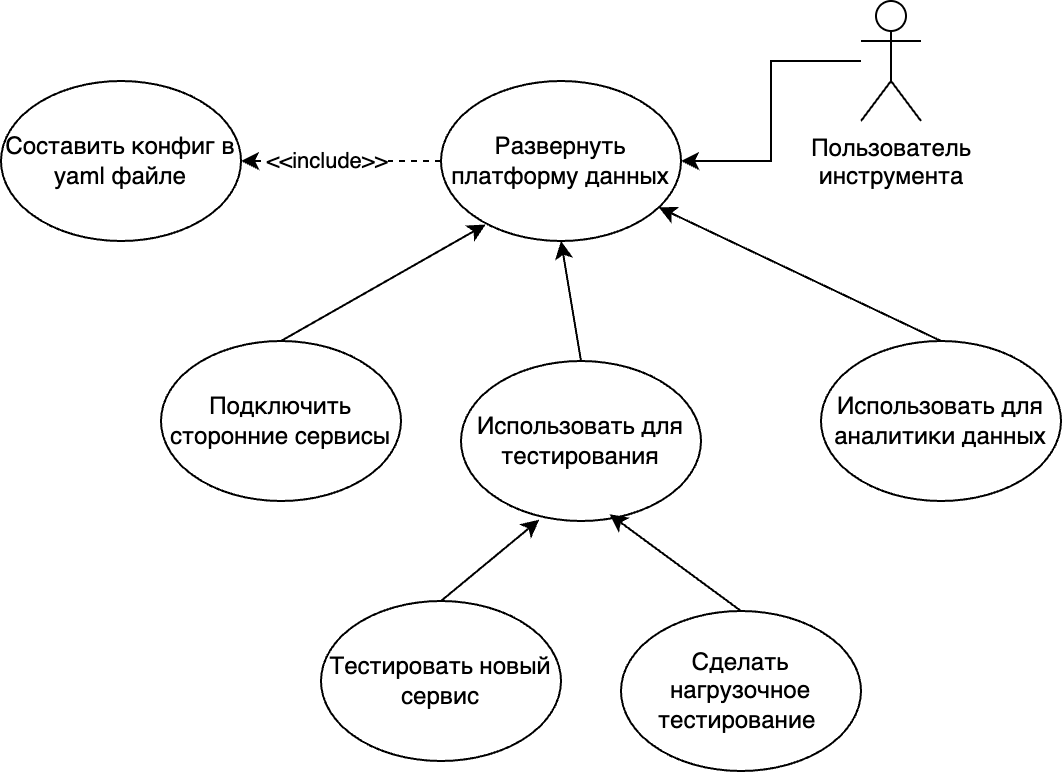
\includegraphics [scale=0.4] {my_folder/images/diagram_usecase}
	\caption{Use-Case диаграмма}
	\label{fig:diagram_usecase}
\end{figure}

% не рекомендуется использовать отдельную section <<введение>> после лета 2020 года
%\section{Введение} \label{ch2:intro}

% Глава посвящена более подробным примерам оформления текстово-графических объектов.

% В параграфе \ref{ch2:title-abbr} приведены примеры оформления многострочной формулы и одиночного рисунка. Параграф \ref{ch2:sec-abbr} раскрывает правила оформления перечислений и псевдокода. В параграфе \ref{ch2:sec-very-short-title} приведены примеры оформления сложносоставных рисунков, длинных таблиц, а также теоремоподобных окружений.


% \section{Название параграфа} \label{ch2:title-abbr} %название по-русски



% %%%%
% %%		
% %%  \input{...} commands are used only to sychronize some parts of the text with the author guide. Authors are free to type the text directly in .tex-files   
% %%  \input{...} комманды используются только, чтобы синхронизировать части текта с рекомендациями авторам. Авторы  вольны вносить текст непосредственно в файл главы  
% %%  
%  \input{my_folder/tex/eq-Galois} % пример двух выравнивания двух формул в окружении align


% На \firef{fig:spbpu-new-bld-autumn-ch2} приведёна фотография Нового научно-исследовательского корпуса СПбПУ.

% 	\begin{figure}[ht] 
% 	\center
% 	\includegraphics [scale=0.27] {my_folder/images/spbpu_new_bld_autumn}
% 	\caption{Новый научно-исследовательский корпус СПбПУ \cite{spbpu-gallery}} 
% 	\label{fig:spbpu-new-bld-autumn-ch2}  
% 	\end{figure}




% \section{Название параграфа} \label{ch2:sec-abbr} %название по-русски

% Название параграфа оформляется с помощью команды \verb|\section{...}|, название главы --- \verb|\chapter{...}|. 


% \subsection{Название подпараграфа} \label{ch2:subsec-title-abbr} %название по-русски


% Название подпараграфа оформляется с помощью команды  \texttt{\textbackslash{}subsection\{...\}}.


% %\subsubsection{Название подподпараграфа} \label{ch2:subsubsec-title-abbr} %название по-русски

% Использование подподпараграфов в основной части крайне не рекомендуется. В случае использования, необходимо вынести данный номер в содержание.	
% Название подпараграфа оформляется с помощью команды  \texttt{\textbackslash{}subsubsecti\-on\{...\}}.



% \input{my_folder/tex/enumeration} % правила использования перечислений	


% Оформление псевдокода необходимо осуществлять с помощью пакета \verb|algorithm2e| в окружении \verb|algorithm|. Данное окружение интерпретируется в шаблоне как рисунок. Пример оформления псевдокода алгоритма приведён на \firef{alg:AlgoFDSCALING}. 


% \input{my_folder/tex/pseudocode-agl-DTestsFDScaling} % пример оформления псевдокода алгоритма 	


% \section{Название параграфа} \label{ch2:sec-very-short-title} %название по-русски



% \input{my_folder/tex/eq-equation-multilined} % пример оформления одиночной формулы в несколько строк

% \input{my_folder/tex/fig-spbpu-sc-four-in-one} % пример подключения 4х иллюстраций в одном рисунке

% %\input{my_folder/tex/fig-spbpu-whitehall-three-in-one} % пример подключения 3х иллюстрации в одном рисунке
% %
% %\input{my_folder/tex/fig-spbpu-main-bld-two-in-one} % пример подключения 2х иллюстраций в одном рисунке

% \input{my_folder/tex/tab-more-than-one-page} % пример подключения таблицы на несколько страциц


% \begin{table} [htbp]% Пример оформления таблицы
% 	\centering\small
% 	\caption{Пример представления данных для сквозного примера по ВКР \cite{Peskov2004}}%
% 	\label{tab:ToyCompare}		
% 		\begin{tabular}{|l|l|l|l|l|l|}
% 			\hline
% 			$G$&$m_1$&$m_2$&$m_3$&$m_4$&$K$\\
% 			\hline
% 			$g_1$&0&1&1&0&1\\ \hline
% 			$g_2$&1&2&0&1&1\\ \hline
% 			$g_3$&0&1&0&1&1\\ \hline
% 			$g_4$&1&2&1&0&2\\ \hline
% 			$g_5$&1&1&0&1&2\\ \hline
% 			$g_6$&1&1&1&2&2\\ \hline		
% 		\end{tabular}
% %	\caption*{\raggedright\hspace*{2.5em} Составлено (или/и рассчитано) по \cite{Peskov2004}} %Если проведена авторская обработка или расчеты по какому-либо источнику	
% 	\normalsize% возвращаем шрифт к нормальному
% \end{table}



% %% please, before using, read the author guide carefully

% \input{my_folder/tex/tab-toy-context-minipage} % пример подключения minipage

% \input{my_folder/tex/fig-spbpu-new-bld-autumn-minipage} % пример подключения minipage




% \input{my_folder/tex/rules-theorem-like-expressions} 

% По аналогии с нумерацией формул, рисунков и таблиц нумеруются и иные текстово-графические объекты, то есть включаем в нумерацию номер главы, например: теорема 3.1. для первой теоремы третьей главы монографии. Команды \LaTeX{} выставляют нумерацию и форматирование автоматически. Полный перечень команд для подготовки текстово-графических и иных объектов находится в подробных методических рекомендациях \cite{spbpu-bci-template-author-guide}. 


% \input{my_folder/tex/rules-list-of-environments} % список некоторых окружений


% \input{my_folder/tex/theorem-example} %пример оформления теоремы


% \input{my_folder/tex/definition-example} %пример оформления определения


% Вместо теоремо-подобных окружений для вставки небольших текстово-графических объектов иногда используются команды. Типичным примером такого подхода является команда \verb|\footnote{text}|\footnote{Внимание! Команда вставляется непосредственно после слова, куда вставляется сноска (без пробела). Лишние пробелы также не указываются внутри команды перед и после фигурных скобок.}, где в аргументе \verb|text| указывают текст \textit{подстрочной ссылки (сноски)}.В них \textit{нельзя добавлять веб-ссылки или цитировать литературу}. Для этих целей используется список литературы. Нумерация сносок сквозная по ВКР без точки на конце выставляется в шаблоне автоматически, однако в каждом приложении к ВКР нумерация, зависящая от номера приложения, выставляется префикс <<П>>, например <<П1.1>> --- первая сноска первого приложения. 




% %\FloatBarrier % заставить рисунки и другие подвижные (float) элементы остановиться


% \section{Выводы} \label{ch2:conclusion}

% Текст заключения ко второй главе. Пример ссылок \cite{Article,Book,Booklet,Conference,Inbook,Incollection,Manual,Mastersthesis,Misc,Phdthesis,Proceedings,Techreport,Unpublished,badiou:briefings}, а также ссылок с указанием страниц, на котором отображены те или иные текстово-графические объекты  \cite[с.~96]{Naidenova2017} или в виде мультицитаты на несколько источников \cites[с.~96]{Naidenova2017}[с.~46]{Ganter1999}. Часть библиографических записей носит иллюстративный характер и не имеет отношения к реальной литературе. 

% Короткое имя каждого библиографического источника содержится в специальном файле \verb|my_biblio.bib|, расположенном в папке \verb|my_folder|. Там же находятся исходные данные, которые с помощью программы \texttt{Biber} и стилевого файла \texttt{Biblatex-GOST} \cite{ctan-biblatex-gost} приведены в списке использованных источников согласно ГОСТ 7.0.5-2008.
% Многообразные реальные примеры исходных библиографических данных можно посмотреть по ссылке \cite{ctan-biblatex-gost-examples}.

% Как правило, ВКР должна состоять из четырех глав. Оставшиеся главы можно создать по образцу первых двух и подключить с помощью команды \verb|\input| к исходному коду ВКР. Далее в приложении \ref{appendix-MikTeX-TexStudio} приведены краткие инструкции запуска исходного кода ВКР \cite{latex-miktex,latex-texstudio}.

% В приложении \ref{appendix-extra-examples} приведено подключение некоторых текстово-графических объектов. Они оформляются по приведенным ранее правилам. В качестве номера структурного элемента вместо номера главы используется <<П>> с номером главы. Текстово-графические объекты из приложений не учитываются в реферате.



%% Вспомогательные команды - Additional commands
%
%\newpage % принудительное начало с новой страницы, использовать только в конце раздела
%\clearpage % осуществляется пакетом <<placeins>> в пределах секций
%\newpage\leavevmode\thispagestyle{empty}\newpage % 100 % начало новой страницы	         	 % Глава 2
\chapter{Разработка инструмента} \label{ch3}

Предварительно важно определить чёткую последовательность этапов,
которая позволит организовать работу над инструментом системно и управляемо.
Это поможет сократить риски неопределенности, оптимально распределить ресурсы и обеспечить своевременный контроль качества на каждом шаге.

Хорошим стилем является наличие введения к главе. Во введении может быть описана цель написания главы, а также приведена краткая структура главы.

\section{План разработки инструмента} \label{ch3:plan_debeloping}
\begin{enumerate}[label=\textbf{Этап \arabic*.}]
      \item Сбор и анализ требований \\
            На этом этапе формализуются функциональные и нефункциональные требования: определяется, какие компоненты Big Data стека поддерживаются, в каком формате задается исходный YAML, какие конфигурационные артефакты должны генерироваться.
      \item  Проектирование архитектуры \\
            Разрабатывается модульная архитектура инструмента, включающая парсер входного описания, генератор промежуточного представления (AST), набор шаблонов для конфигураций инструментов и механизм их объединения в итоговые файлы. Определяются границы ответственности каждого модуля, протокол взаимодействия между ними и формат плагинов для расширения функциональности.
      \item  Определение языка декларативного описания \\
            Уточняются синтаксис и семантика входного YAML: структура разделов, типы параметров, возможные зависимости и проверки корректности. Разрабатывается схема jsonschema для валидации пользовательских описаний на раннем этапе.
      \item  Реализация ядра: парсер и промежуточное представление \\
            Пишется компонент, который читает декларативный файл, проводит его валидацию по схеме (jsonschema), конструирует внутреннее дерево объектов (AST) с отображением всех сущностей и их связей. Этот модуль обеспечивает основу для дальнейших операций по генерации конфигураций.
      \item Разработка генераторов конфигурационных файлов \\
            На основе AST реализуются плагины-генераторы для каждого типа артефакта:
            \begin{itemize}
                  \item docker-compose.yaml с сервисами и сетями;
                  \item Конфигурации PostgreSQL (postgresql.conf, init.sql);
                  \item JSON-файлы коннекторов Debezium и S3Sink;
                  \item Файлы настроек для ClickHouse;
                  \item Конфигурационные файлы для AKHQ и Superset.
            \end{itemize}
            Каждый генератор использует шаблонизатор и преобразует параметры из AST в конкретные строки и блоки файлов.
      \item Создание CLI-интерфейса\\
            Реализуется утилита командной строки, позволяющая пользователю запускать генерацию: передавать путь к входному файлу,  указывать директорию вывода, включать опции валидации и отладки. CLI обеспечивает удобство использования инструмента в скриптах и CI/CD-пайплайнах\cite{acid}.
      \item Модуль тестирования и валидации\\
            Пишутся автоматические тесты: модульные тесты для парсера и генераторов, интеграционные — для проверки корректного результата генерации по ряду типовых YAML-конфигураций. Добавляются проверки на соответствие с эталонными файлами и на корректность в Docker-среде (например, пробный запуск docker-compose up).
      \item Документирование и примеры\\
            Готовится подробная документация: описание формата входного файла, руководство пользователя CLI, схемы и примеры конфигураций «из коробки» для типовых сценариев (EDW на PostgreSQL→Kafka→ClickHouse→Superset). Включаются рекомендации по расширению и отладке.
      \item Пилотное развертывание и сбор обратной связи\\
            Инструмент разворачивается в тестовой среде или локально на реальных примерах, собираются отзывы от пользователей — инженеров и аналитиков. На основе полученных замечаний корректируются шаблоны, схемы и UX CLI.
      \item Релиз и сопровождение\\
            Формируется релизная сборка, обеспечивается публикация в открытый репозиторий GitHub, настраивается процесс выпуска обновлений и приёма issue. Определяется модель поддержки: дорожная карта, приоритеты новых возможностей и исправлений.
\end{enumerate}


\section{Язык декларативного описания (DSL)} \label{ch3:dsl}
Практический опыт показывает, что повышение уровня абстракции и учёт специфики предметной области наиболее эффективно достигаются через разработку собственного языка предметной области - Domain Specific Language, DSL\cite{novikov_grammatik}\cite{ulman}. Такой язык представляет собой формальный аппарат, работающий непосредственно с понятиями и структурами предметной области, позволяя лаконично формулировать и решать большинство типовых задач.

В нашем случае DSL строится на основе YAML\cite{yaml} – удобного человеко-ориентированного формата сериализации, концептуально схожего с языками разметки, но оптимизированного для записи и чтения распространённых структур данных.


Ключевые особенности синтаксиса YAML:
\begin{enumerate}[1.]
      \item Отступы и вложенность\\
            Используются только пробелы (обычно 2 или 4) для обозначения уровней вложенности. Символ табуляции запрещён.
      \item Пары «ключ–значение»\\
            Каждая запись имеет вид ключ: значение, где после двоеточия обязательно идёт пробел.
      \item Списки\\
            Элементы маркируются дефисом и пробелом (- элемент).
      \item Многострочные литералы\\
            Символ | сохраняет все разрывы строк. Символ > объединяет строки, заменяя отступы и разрывы единичными пробелами.
      \item Якоря и ссылки\\
            Якорь (\&имя) позволяет дать имя блоку значений. Ссылка (*имя) повторно вставляет ранее объявленный блок.\\
            Пример:
\end{enumerate}

\begin{verbatim}
        default: &base
        имя: Oleg
        возраст: 27

        user_2:
        <<: *base
\end{verbatim}
Чтобы формализовать синтаксис DSL и задать конечное описание потенциально
бесконечного множества допустимых конфигураций,
мы опираемся на контекстно-свободную грамматику $G=\langle N,T,R,S\rangle$, где:\\
$N$ – множество нетерминальных символов \\
$T$ – терминальные (т. е. реальные лексемы) \\
$R$ – правило вида $A$→$\alpha$ (замена нетерминала A на строку символов $\alpha$) \\
$S$ – стартовый нетерминал.

По классификации Хомского такая грамматика относится ко второму типу (КСГ): в каждом правиле слева стоит ровно один нетерминал, который может быть заменён на любую допустимую цепочку из  $A\cup B$.

Реализация парсера и генератора AST (абстрактного синтаксического дерева) опирается на ANTLR (ANother Tool for Language Recognition)\cite{antlr_lab}.
Лексические правила (начинаются с большой буквы) описывают, как разбить входной текст на токены.
Пример:\\
\begin{verbatim}
// Лексическое правило для целых чисел
INT : [0-9]+ ; 
\end{verbatim}
Синтаксические правила (начинаются с маленькой буквы) задают структуры из токенов.
Пример:
\begin{verbatim}
// Синтаксическое правило для списка аргументов
args : expr (',' expr)* ; 
\end{verbatim}
Для группировки, повторений и альтернатив в ANTLR применяются:\\
«()» – группировка\\
«*» – 0 или более повторений\\
« +» – 1 или более\\
«?» – 0 или 1 раз\\
« |» – выбор одной из альтернатив\\
«:» и «;» – разделители начала и конца правил.\\

Описание языка DPD (Data Platform Deployer)

Язык DPD  разработан для  декларативного описания архитектуры платформы данных единым удобным форматом и автоматической генерации всех необходимых инструментов для быстрого развертывания и тестирования готового стенда. В общих чертах имеет следующую структуру:
\begin{verbatim}
project:
    name: data-platform-14
    version: 1.2.0
    description: This is a project for testing data platform
sources:
    - type: postgres
    name: postgres_1
    - type: postgres
    name: postgres_2
    - type: s3
    name: s3_1
streaming:
    kafka:
        num_brokers: 3
    connect:
        name: connect-1
storage:
    clickhouse:
    name: clickhouse-1
bi:
    superset:
    name: superset-1
\end{verbatim}
В приложении \ref{grammatic-dpd}  приведена часть полной грамматики, описывающая правила в форме ANTLR \\



% \FloatBarrier % заставить рисунки и другие подвижные (float) элементы остановиться


\section{Описание процесса автогенерации конфигураций программных систем платформы данных} \label{ch3:process_generation}
Архитектура инструмента в значительной степени повторяет логическое разбиение на блоки, которое представлено в начале этой главы.

Пакет \texttt{data platform} взаимодействует с пакетом \texttt{core}, внутри которого как раз таки находятся парсер, генератор, сервисы, а также другие дополнительные элементы.
Диаграмма представлена на рисунке \ref{fig:diagram_package}

\begin{figure}
      \center
      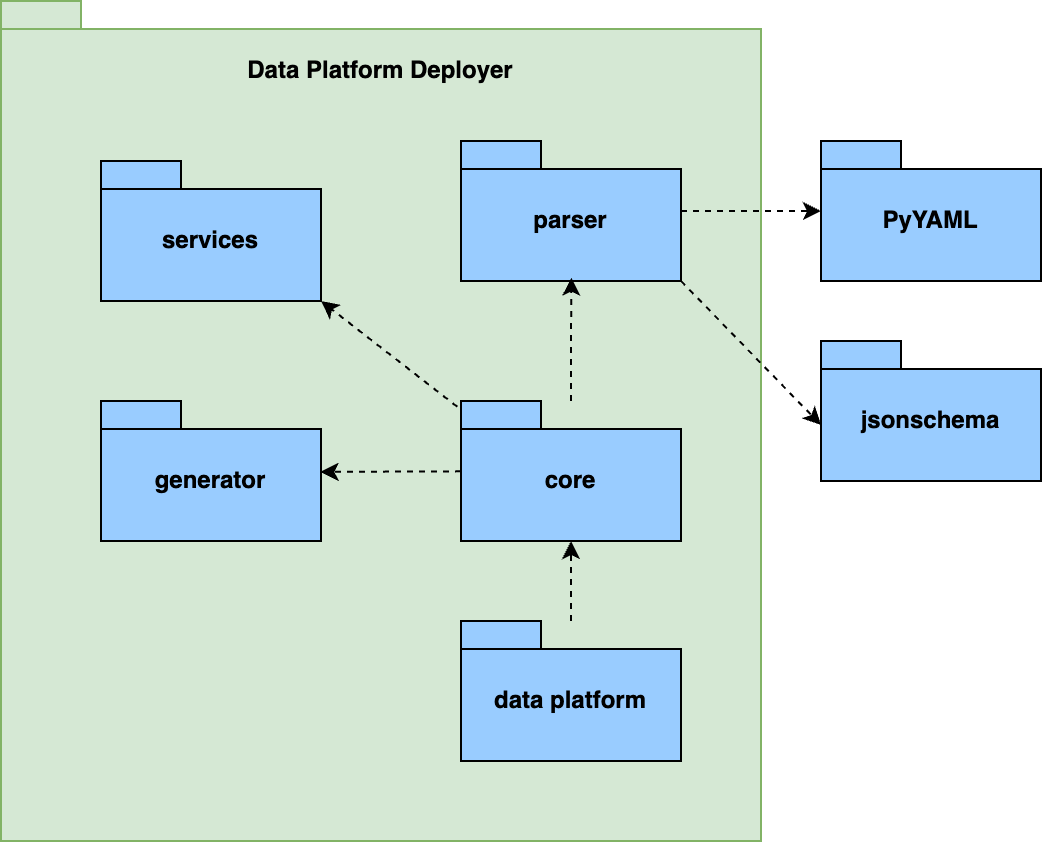
\includegraphics [scale=0.4] {my_folder/images/diagram_package}
      \caption{Диаграмма пакетов}
      \label{fig:diagram_package}
\end{figure}
\FloatBarrier
Стоит детальнее рассмотреть содержимое пакета \texttt{core}, ведь именно там выполняется генерация конфигураций программных систем платформы данных.
Процесс автоматической генерации конфигураций для платформы данных с использованием инструмента \texttt{dpd} можно разделить на следующие ключевые этапы:
\begin{enumerate}[1.]

      \item Инициация через командную строку (\texttt{main.py})
            \begin{itemize}
                  \item \textbf{Входная точка.} Пользователь взаимодействует с инструментом через CLI, вызывая основную команду \texttt{dpd}.
                  \item \textbf{Команда \texttt{generate}.} Логика запускается командой
                        \texttt{dpd generate} с обязательным параметром
                        \texttt{--config <путь\_к\_YAML>}.
                  \item \textbf{Оркестрация.} Файл \texttt{main.py} парсит аргументы командной строки, вызывает функции валидации и загрузки конфигурации, инициализирует генератор платформы и запускает процесс, выводя информативные сообщения.
            \end{itemize}

      \item Валидация и загрузка конфигурации (\texttt{main.py} \textrightarrow\ \texttt{dpd.models}):
            \begin{itemize}
                  \item \textbf{Проверка схемы.} Перед генерацией выполняется валидация YAML-конфига по JSON-схеме (\texttt{src/dpd/schema.json}) с помощью функции \texttt{validate} из \texttt{dpd.models} и библиотеки \texttt{jsonschema}.
                  \item \textbf{Загрузка и моделирование.} При успешной валидации содержимое конфигурации загружается и преобразуется в Python-модели (\texttt{Config}, \texttt{Postgres}, \texttt{S3} и т.~п.) через функцию \texttt{load\_config\_from\_file}.
            \end{itemize}

      \item Инициализация генератора платформы (\texttt{main.py} \textrightarrow\ \texttt{data\_platform.py})
            \begin{itemize}
                  \item \textbf{Создание \texttt{DPGenerator}.} В конструктор передаётся смоделированная конфигурация (\texttt{conf}).
                  \item \textbf{Начальное состояние.} Генератор инициализирует пустые словари для сервисов и настроек, создаёт описание сетей Docker на основе имени проекта, подготавливает \texttt{PortManager} и \texttt{EnvManager}.
            \end{itemize}

      \item Обработка сервисов и делегирование (\texttt{DPGenerator.process\_services})
            \begin{itemize}
                  \item \textbf{Итерация.} Метод перебирает секции конфигурации (\texttt{sources}, \texttt{streaming}, \texttt{storage}, \texttt{bi}).
                  \item \textbf{Делегирование.} В зависимости от компонента (\texttt{postgres}, \texttt{s3}, \texttt{kafka}, \texttt{clickhouse}, \texttt{superset}) вызываются соответствующие статические методы \texttt{generate()} из модулей \texttt{dpd.services}.
                  \item \textbf{Сборка.} Каждый сервис генерирует свой блок для \texttt{docker-compose.yml} и вспомогательные файлы, результат добавляется в словарь \texttt{self.services}.
                  \item \textbf{Зависимости.} Для некоторых генераций (например, \texttt{KafkaConnectService}) учитываются заранее созданные компоненты (Postgres-источники и т.~п.).
            \end{itemize}

      \item Генерация вспомогательных файлов
            \begin{itemize}
                  \item \textbf{README.md.} \texttt{ReadmeService.generate\_file()} создаёт описание платформы и инструкции.
                  \item \textbf{.env.} \texttt{EnvManager.generate\_env\_file()} помещает все секреты (пароли, ключи) в файл \texttt{.env}.
                  \item \textbf{init.sql.} \texttt{PostgresqlService.generate\_init\_sql\_script()} формирует SQL-скрипт для инициализации (создание публикации, репликационные слоты).
                  \item \textbf{postgresql.conf.} \texttt{PostgresqlService.generate\_conf\_file()} генерирует конфигурацию WAL (напр., \texttt{wal\_level}, \texttt{max\_wal\_senders}, \texttt{max\_replication\_slots}).
                  \item \textbf{Конфигурации Debezium и S3SinkConnector.} Функции \texttt{generate\_debezium\_configs()} и \texttt{generate\_s3sink\_configs()} создают JSON-файлы для репликации Postgres→Kafka и Kafka→S3, которые затем загружаются в Kafka Connect через REST API.
                  \item \textbf{Плагины для Kafka Connect.} Автоматически скачиваются JAR-файлы S3SinkConnector и ClickHouseConnector.
                  \item \textbf{AKHQ.} \texttt{KafkaUIService.generate\_conf\_file()} связывает веб-интерфейс AKHQ с кластерами Kafka и Kafka Connect.
            \end{itemize}

      \item Сборка и запись итогового файла
            \begin{itemize}
                  \item \textbf{Формирование структуры.} Метод \texttt{generate()} собирает все настройки, описания сервисов, тома (метод \texttt{\_generate\_volumes()}) и сети в единый Python-словарь, соответствующий формату \texttt{docker-compose.yml}.
                  \item \textbf{Сериализация.} Структура преобразуется в YAML при помощи \texttt{PyYAML}.
                  \item \textbf{Запись.} Итоговый YAML записывается в файл \texttt{docker-compose.yml} в директории с именем проекта. Директория создаётся автоматически при необходимости.
            \end{itemize}
\end{enumerate}

Таким образом, инструмент \texttt{dpd} берёт на вход декларативное описание платформы данных, проверяет его, последовательно генерирует конфигурации для каждого компонента и собирает их в готовый к запуску стек под управлением Docker Compose, а также создаёт сопутствующие файлы (\texttt{README.md}, \texttt{.env}, \texttt{postgresql.conf}, \texttt{dbz\_conf.json}, \texttt{s3\_sink.json}, \texttt{akhq\_conf.yml} и др.).


% Текст выводов по главе \thechapter.


%% Вспомогательные команды - Additional commands
%
%\newpage % принудительное начало с новой страницы, использовать только в конце раздела
%\clearpage % осуществляется пакетом <<placeins>> в пределах секций
%\newpage\leavevmode\thispagestyle{empty}\newpage % 100 % начало новой страницы           	 % Глава 3
\chapter{Проектирование и реализация инфраструктуры программных системы для работы с большими данными} \label{ch4}

% не рекомендуется использовать отдельную section <<введение>> после лета 2020 года
%\section{Введение} \label{ch4:intro}

% Хорошим стилем является наличие введения к главе. Во введении может быть описана цель написания главы, а также приведена краткая структура главы. 
Весь процесс проектирования можно иллюстрировать следующей диаграммой активности (\firef{fig:diagram_activity})

\begin{figure}
  \center
  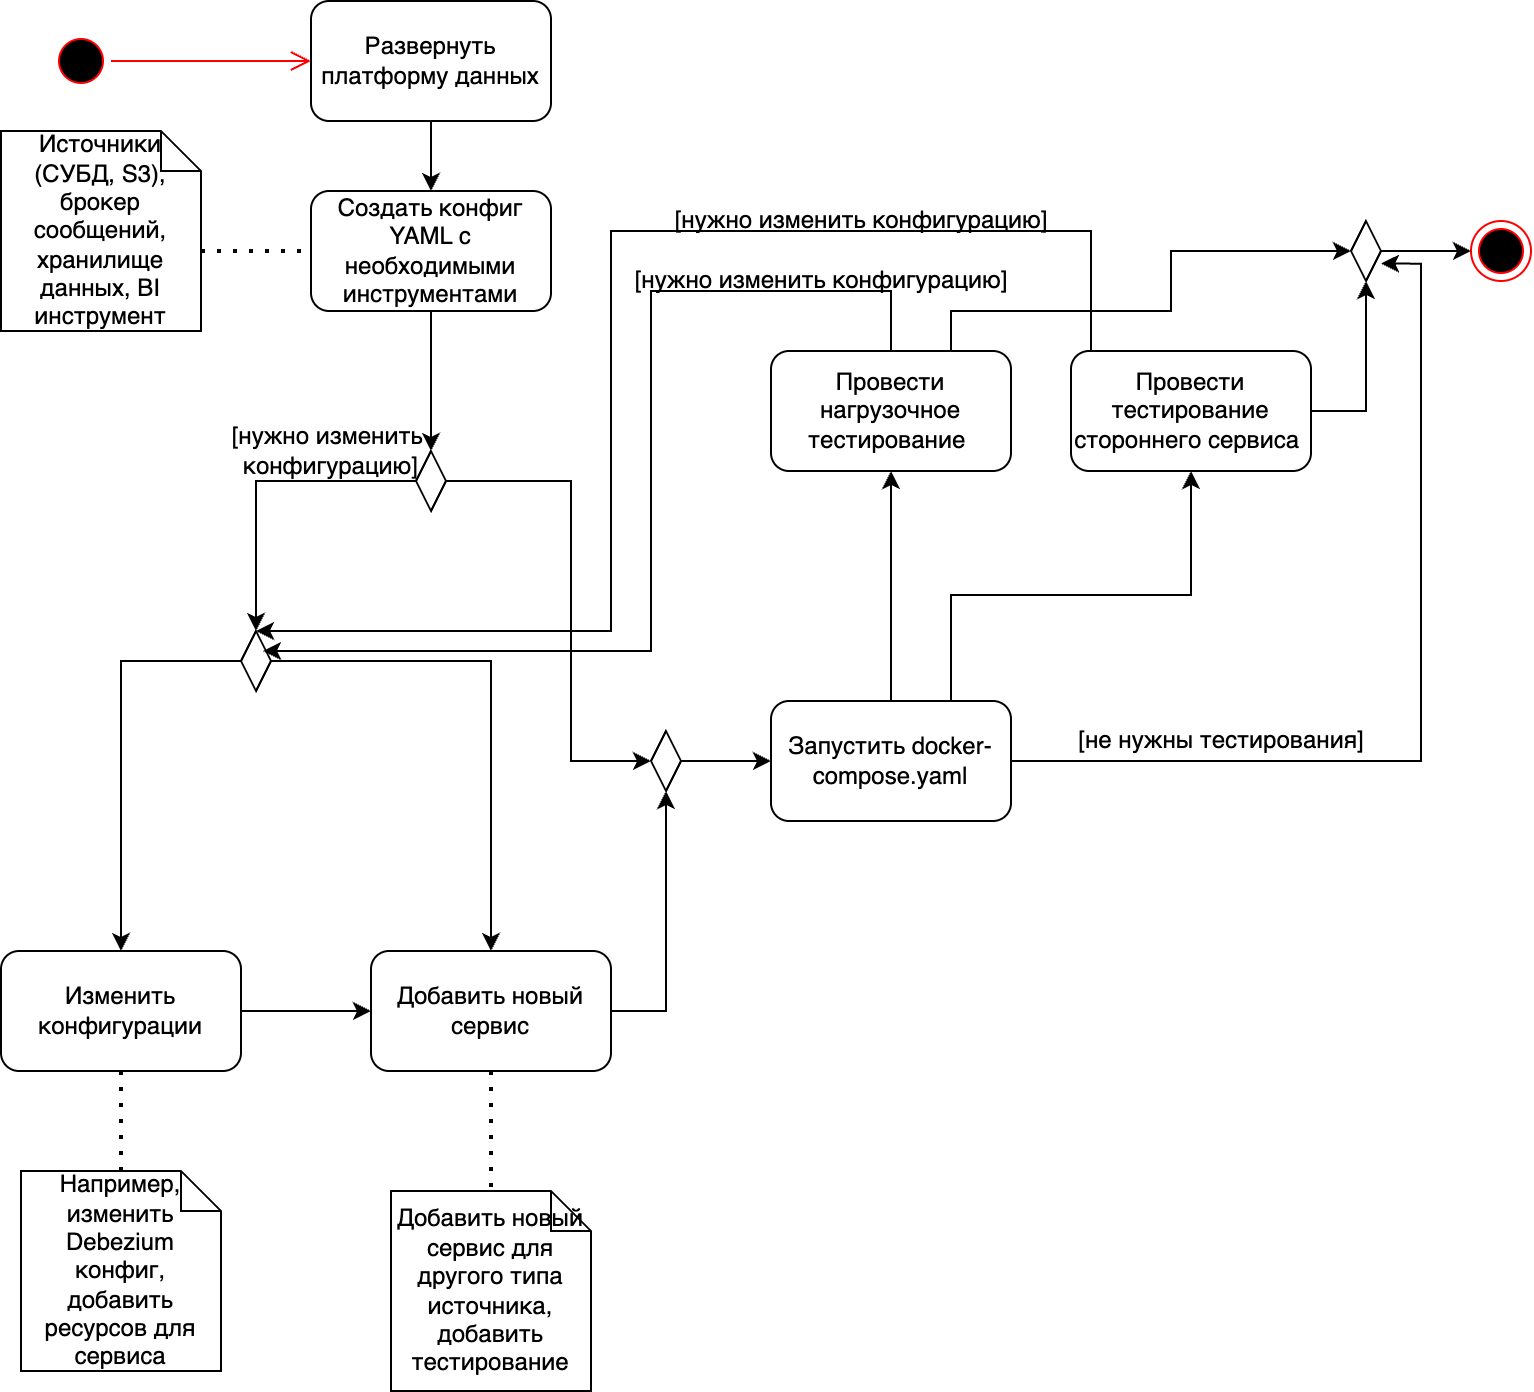
\includegraphics [scale=0.3] {my_folder/images/diagram_activity}
  \caption{Диаграмма пакетов}
  \label{fig:diagram_activity}
\end{figure}
\FloatBarrier
В данном разделе будут рассмотрены практические примеры использования инструмента для развертывания полноценных платформ данных. На примере двух известных датасетов, Northwind\cite{northwind} и Chinook\cite{chinook}, будет продемонстрирован весь цикл настройки и работы конвейера данных: от источников до систем хранения и визуализации. Эти примеры иллюстрируют, как с помощью декларативной конфигурации можно быстро построить и запустить сложную инфраструктуру для анализа данных.



\section{Пример Northwind: Связь клиентов с заказами} \label{ch4:northwind}
Данный пример демонстрирует полный цикл обработки данных с использованием платформы, сгенерированной инструментом dpd на основе простой конфигурации. В качестве источника используется классический датасет "Northwind"\cite{northwind}, загруженный в СУБД PostgreSQL.

Цель – показать, как данные из операционной базы данных проходят через систему потоковой обработки Kafka, сохраняются в аналитическом хранилище ClickHouse и визуализируются с помощью BI-инструмента Superset. Параллельно данные также архивируются в S3-совместимое хранилище Minio.

\begin{enumerate}[1.]
  \item Конфигурация платформы\\
        Для генерации инфраструктуры использовался следующий конфигурационный файл \texttt{config.yaml}:
        \begin{verbatim}
project:
  name: data-platform-northwind 
  version: 1.0.0
  description: Northwind end-to-end
sources:
  - type: postgres
    name: postgres_1
  - type: postgres
    name: postgres_2 # Дополнительный источник
  - type: s3
    name: s3_1      # S3-совместимое хранилище (Minio)
streaming:
  kafka:
    num_brokers: 6
  connect:
    name: connect-1 
storage:
  clickhouse:
    name: clickhouse-1 # Аналитическое хранилище
bi:
  superset:
    name: superset-1 # BI-инструмент  
\end{verbatim}

  \item Развертывание и статус сервисов\\
        После запуска команды \texttt{dpd generate ---config config.yaml} был создан файл \texttt{docker-compose.yml} и сопутствующие конфигурации. Платформа была развернута стандартной командой \texttt{docker compose up -d}. Все сервисы (PostgreSQL, Minio, Kafka-брокеры, Kafka Connect, Kafka UI, ClickHouse, Superset) успешно запустились и работали в штатном режиме(\firef{fig:ex1_docker_services}).
        \clearpage
        \begin{figure}[h]
          \center
          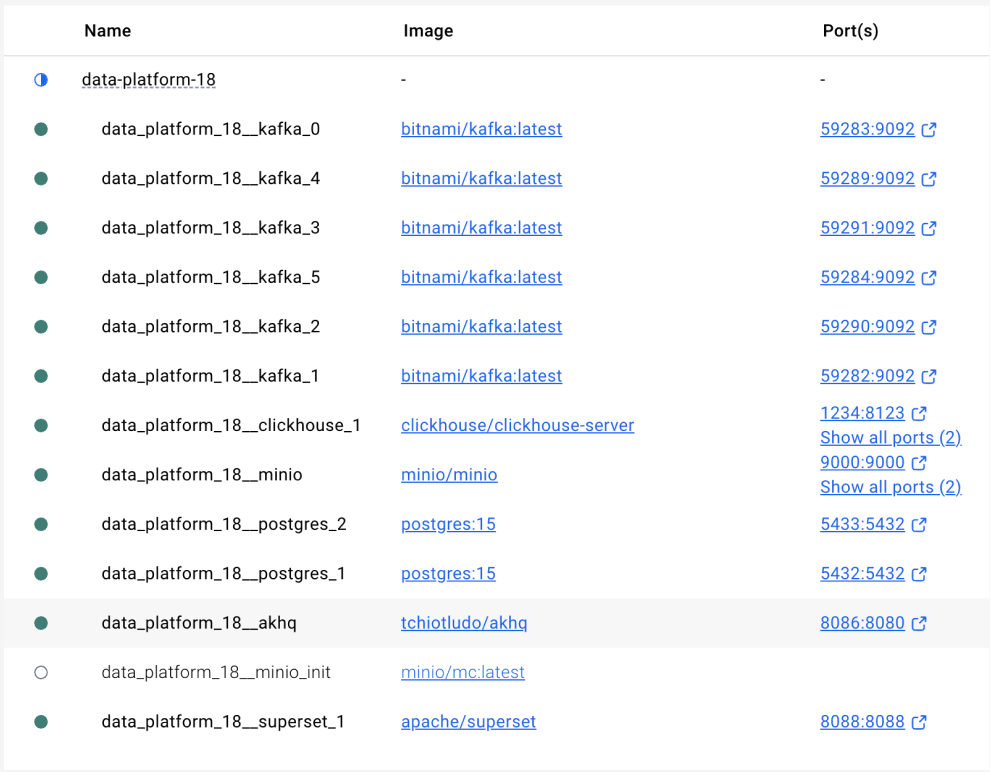
\includegraphics [scale=0.4] {my_folder/images/ex1_docker_services.png}
          \caption{ Статус сервисов в Docker Desktop}
          \label{fig:ex1_docker_services}
        \end{figure}
        \clearpage
        \FloatBarrier
  \item Поток данных от источника до BI
        \begin{itemize}
          \item Источник данных (PostgreSQL)\\
                База данных Northwind была предварительно загружена в экземпляр PostgreSQL. DDL базы Northwind изображена на рисунке \ref{fig:ex1_schema_ddl}
                \begin{figure}[h]
                  \center
                  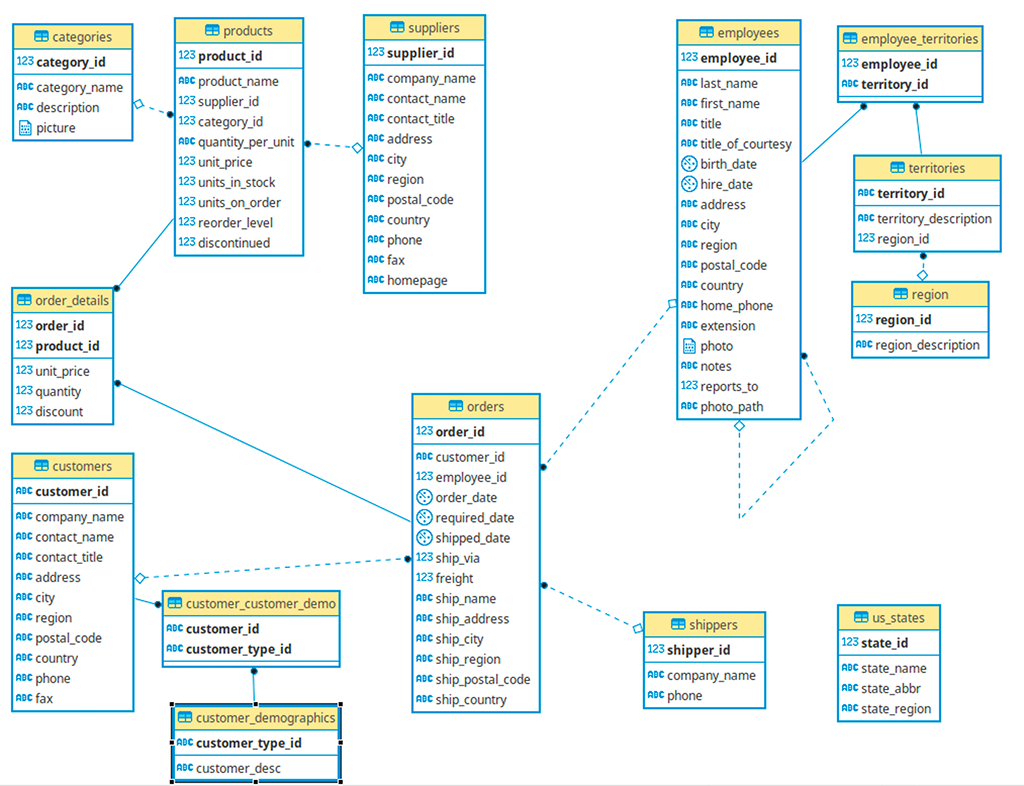
\includegraphics [scale=0.8] {my_folder/images/ex1_schema_ddl}
                  \caption{DDL схемы Northwind в PostgreSQL}
                  \label{fig:ex1_schema_ddl}
                \end{figure}
          \item Захват изменений (Debezium + Kafka Connect):\\
                Для отслеживания изменений (операций INSERT, UPDATE, DELETE) в таблицах PostgreSQL были автоматически созданные коннекторы Debezium PostgreSQL и S3SinkSourceConnector, работающий внутри сервиса Kafka Connect. Коннектор читает WAL (Write-Ahead Log) базы данных и публикует все изменения в виде сообщений в соответствующие топики Apache Kafka. Для каждой таблицы был автоматически создан свой топик.
                \begin{figure}[h]
                  \center
                  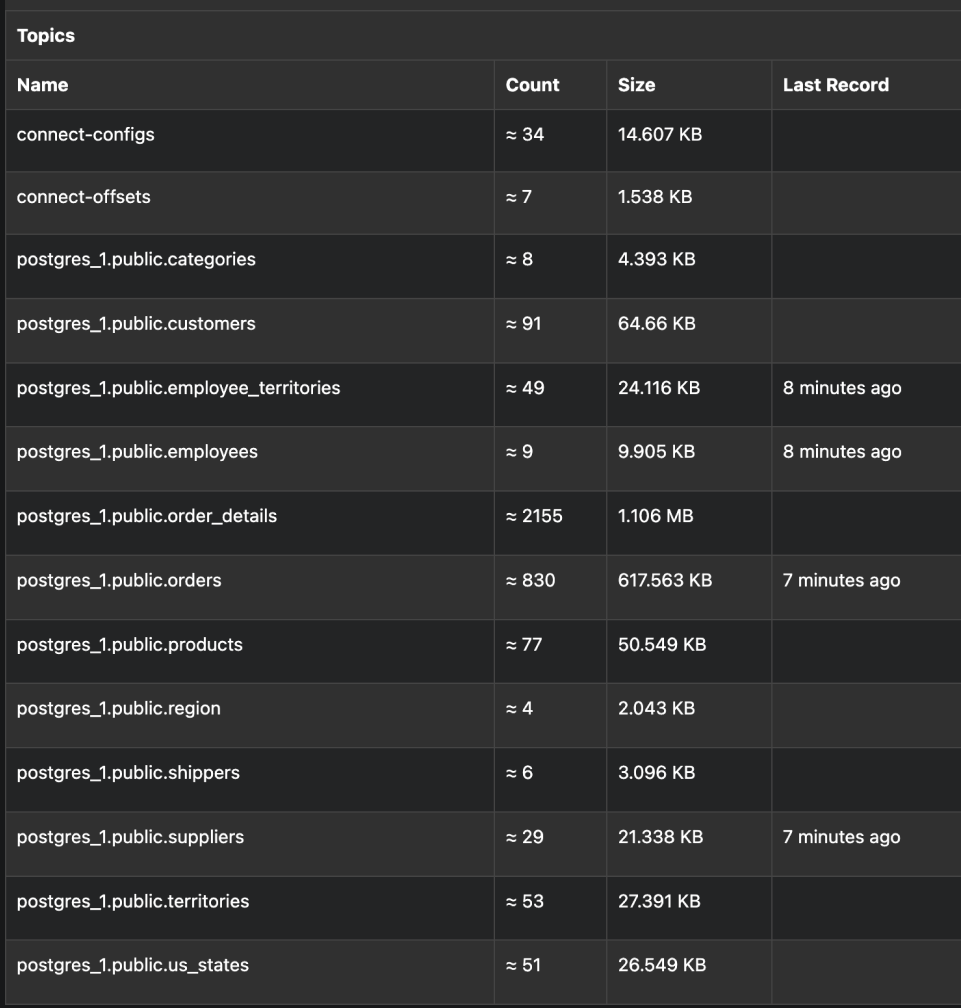
\includegraphics [scale=0.3] {my_folder/images/ex1_kafka_topics}
                  \caption{Список активных Kafka-топиков в Kafka UI}
                  \label{fig:ex1_kafka_topics}
                \end{figure}
                \FloatBarrier
                \begin{figure}[h]
                  \center
                  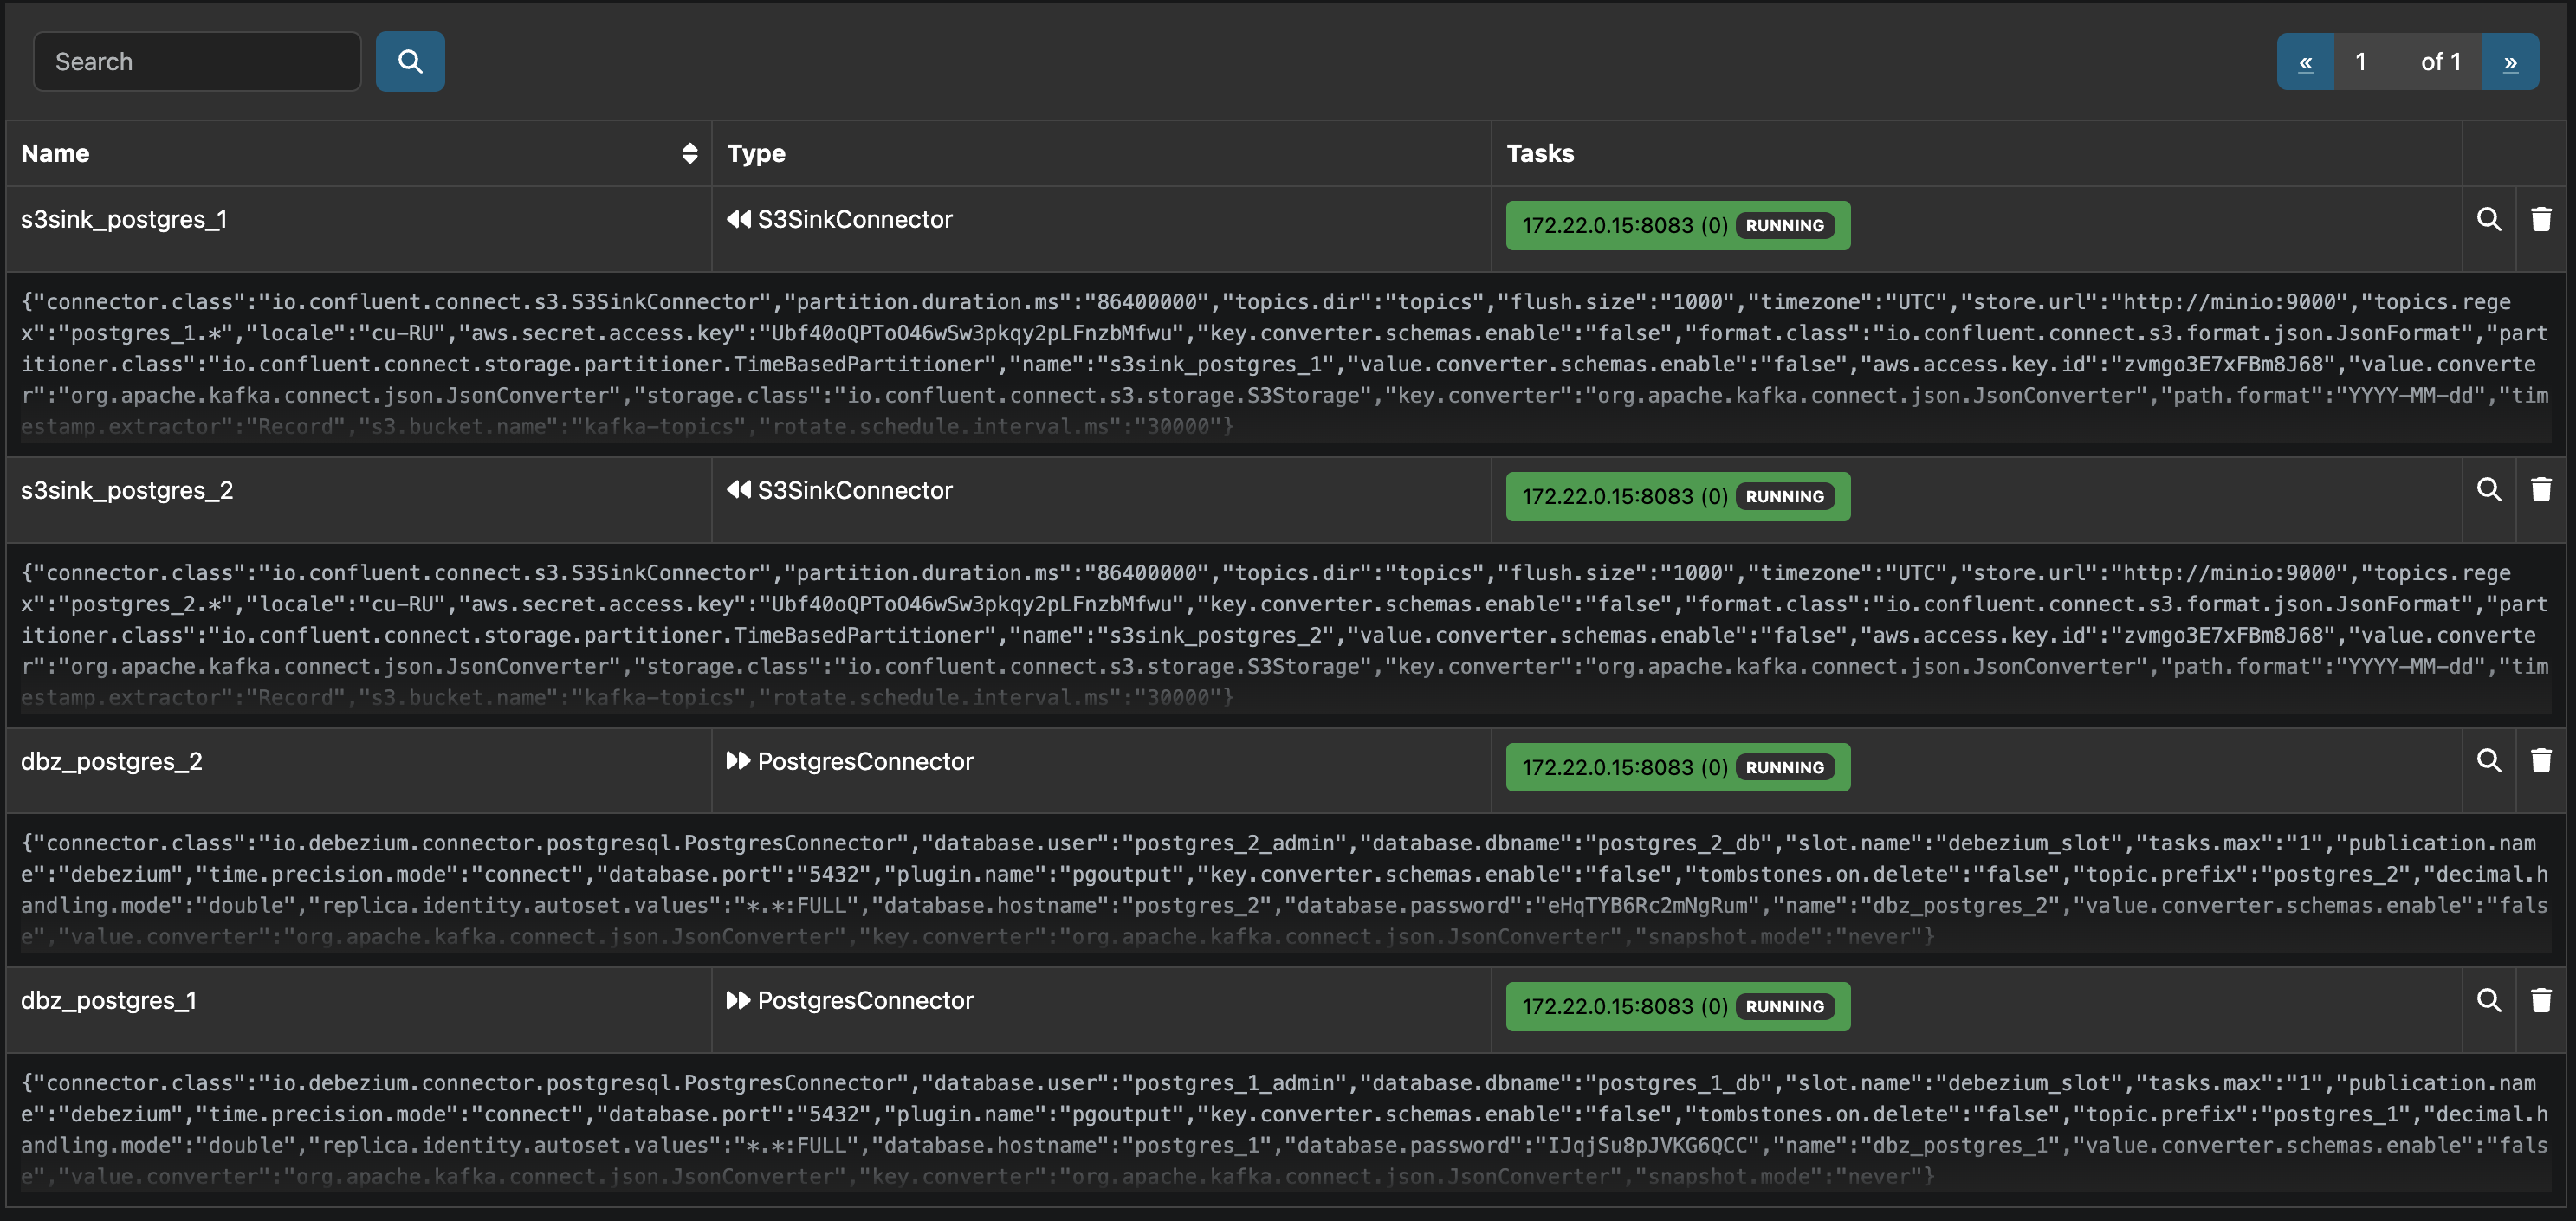
\includegraphics [scale=0.3] {my_folder/images/ex1_kafka_connectors}
                  \caption{Коннекторы в Kafka UI}
                  \label{fig:ex1_kafka_connectors}
                \end{figure}
                \FloatBarrier
          \item Загрузка в аналитическое хранилище (ClickHouse):\\
                Данные из Kafka доставлялись в ClickHouse с использованием встроенного движка KafkaEngine. Для каждой таблицы источника была создана связка:
                \begin{enumerate}[1.]
                  \item Таблица на движке KafkaEngine\cite{clickhouse}, которая подписывается на соответствующий топик Kafka и читает из него сообщения "на лету".
                  \item Целевая таблица на движке MergeTree\cite{clickhouse} для эффективного хранения и аналитических запросов.
                  \item Материализованное представление, которое автоматически считывает данные из Kafka-таблицы и вставляет их в MergeTree-таблицу, выполняя при необходимости базовые преобразования.
                \end{enumerate}
                Пример SQL кода для забора данных из Kafka в ClickHouse для таблицы \texttt{orders} находится в приложении \ref{ex_1_sql}
                \begin{figure}[h]
                  \center
                  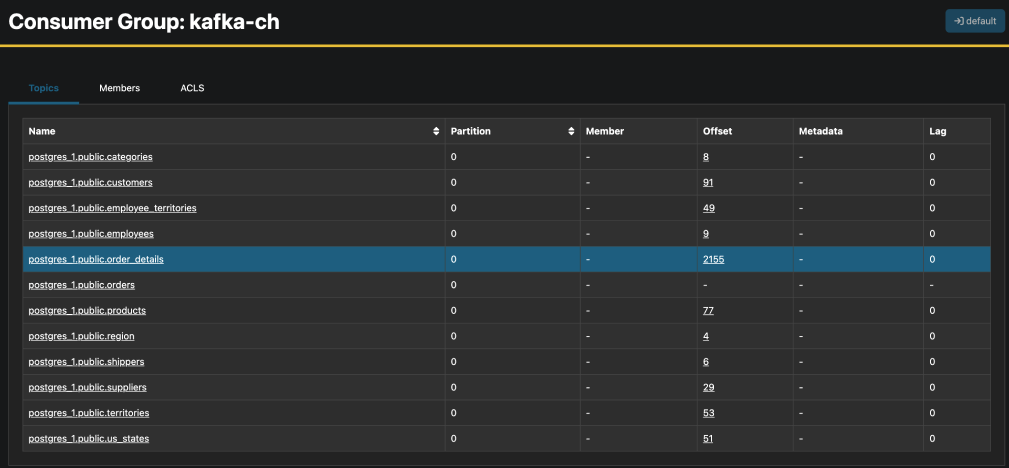
\includegraphics [scale=0.45] {my_folder/images/ex1_kafka_ch_consumer}
                  \caption{Группы консьюмеров ClickHouse в Kafka UI}
                  \label{fig:ex1_kafka_ch_consumer}
                \end{figure}
                \FloatBarrier
          \item Архивация данных в S3\\
                Параллельно с основной обработкой, данные из Kafka-топиков архивировались
                в S3-хранилище (реализованное через Minio). Kafka Connect S3 Sink Connector считывал сообщения
                из топиков и сохранял их в виде файлов JSON в соответствующие директории внутри S3 бакета(рис \ref{fig:ex1_s3}). Это обеспечивает долговременное хранение сырых данных.
                \begin{figure}[h]
                  \center
                  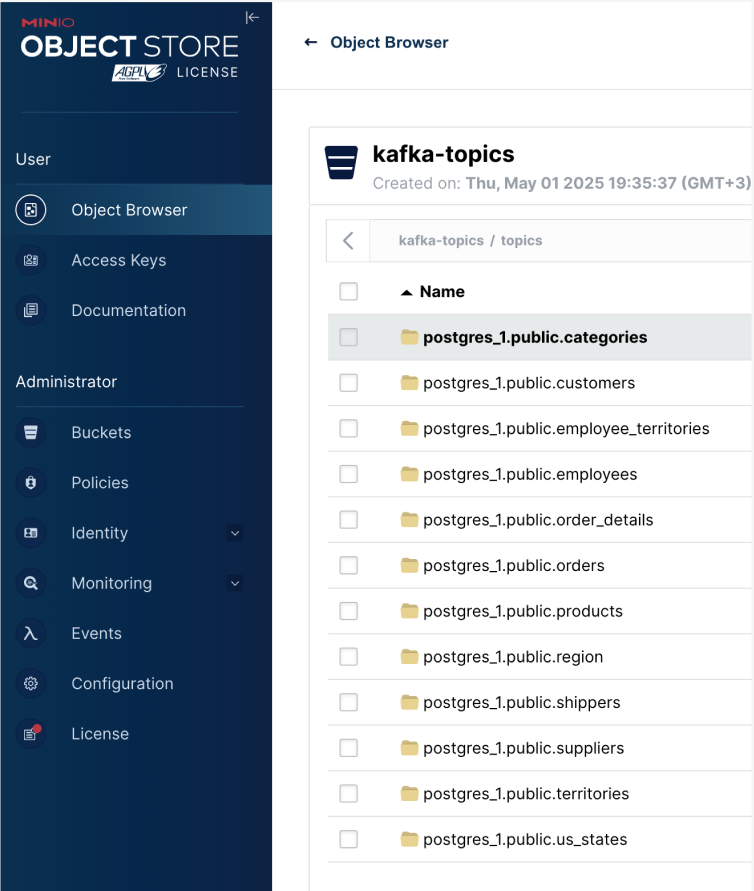
\includegraphics [scale=0.45] {my_folder/images/ex1_s3}
                  \caption{ Список директорий в S3, соответствующих топикам Kafka}
                  \label{fig:ex1_s3}
                \end{figure}
                \FloatBarrier
          \item Загрузка и хранение в ClickHouse\\
                Данные о продажах и связанных сущностях доставлялись из Kafka в ClickHouse с использованием стандартного паттерна c предыдущего примера: Kafka Engine таблица для чтения из топика и Materialized View для переноса данных в целевую таблицу на движке MergeTree. Это позволило эффективно хранить данные для аналитических запросов.
          \item Проверка целостности данных\\
                Было проведено сравнение количества записей в ключевых таблицах источника (PostgreSQL) и приемника (ClickHouse). Сравнение показало полное совпадение количества строк, что свидетельствует об успешной и полной доставке данных.
                \begin{figure}[h]
                  \center
                  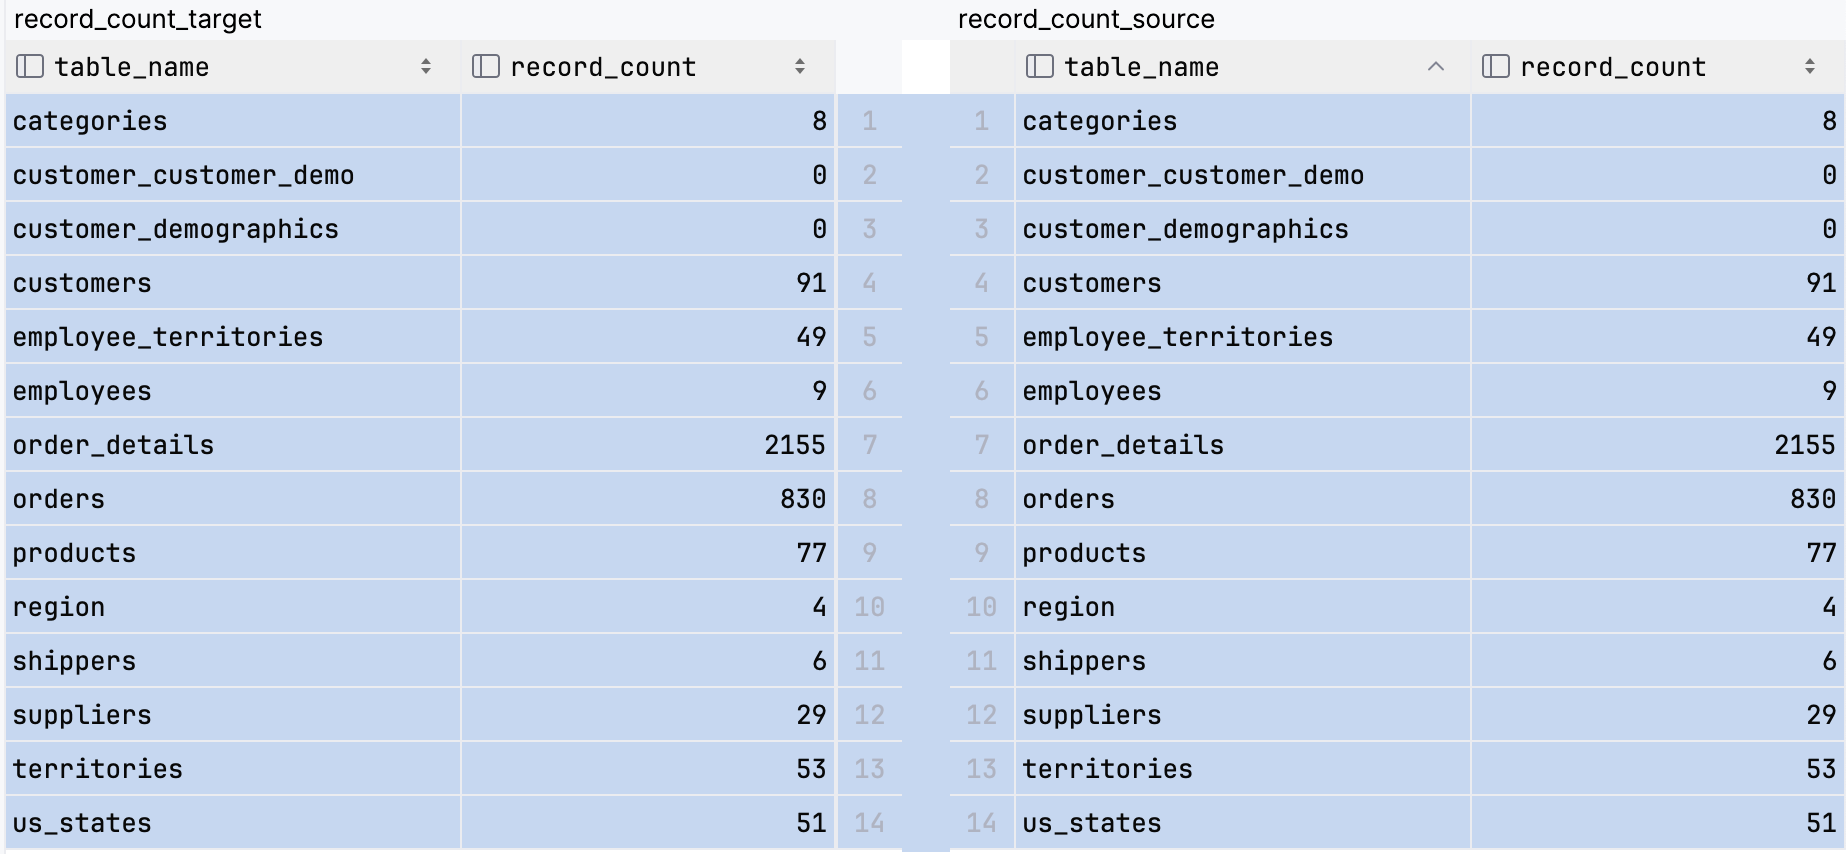
\includegraphics [scale=0.5] {my_folder/images/ex1_tables_ch_pg_compraring}
                  \caption{Сравнение количества строк в PostgreSQL и ClickHouse для Northwind}
                  \label{fig:ex1_tables_ch_pg_compraring}
                \end{figure}
                \FloatBarrier
          \item Анализ и Визуализация (Superset)\\
                Данные, загруженные в ClickHouse, были подключены как источник в Apache Superset. На основе этих данных был построен дашборд, включающий визуализацию, например, график среднего времени обработки заказа по месяцам(\firef{fig:ex1_superset_chart}). Это демонстрирует готовность данных к анализу и построению отчетности.                    \begin{figure}[h]
                  \center
                  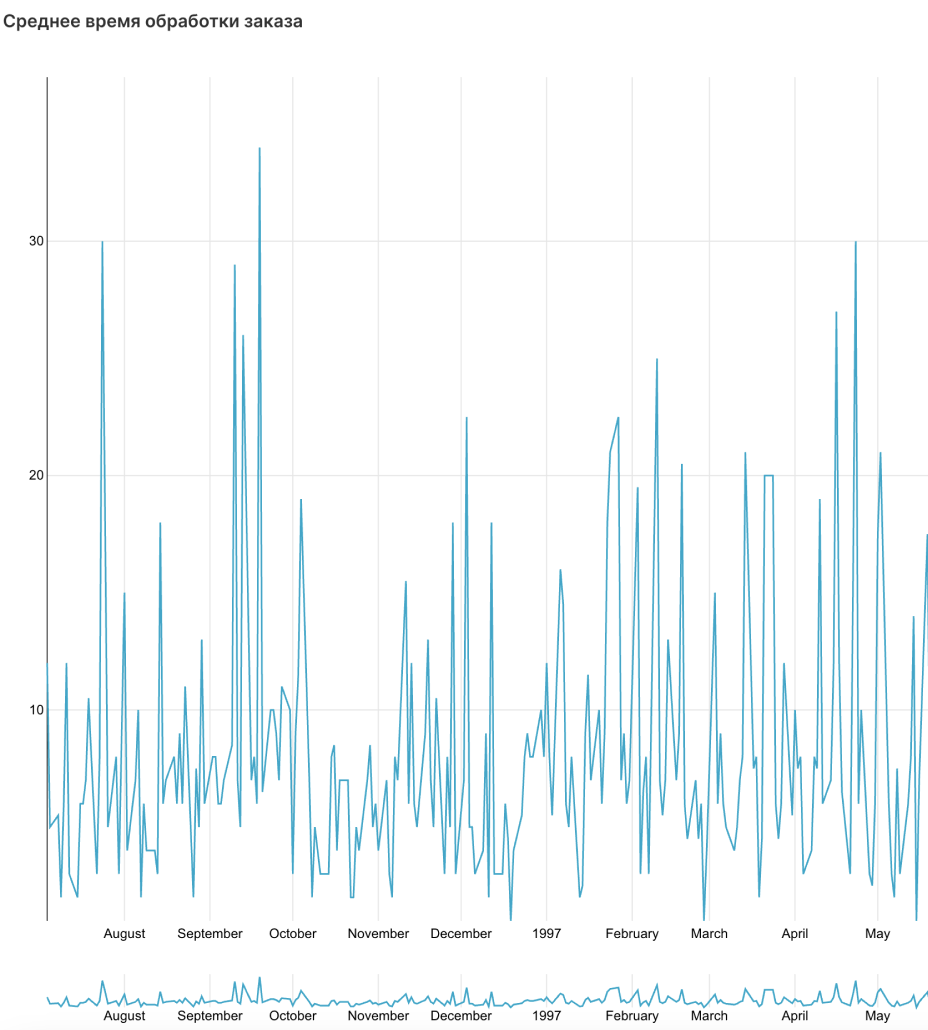
\includegraphics [scale=0.45] {my_folder/images/ex1_superset_chart}
                  \caption{Чарт в Superset "Среднее время обработки заказа"}
                  \label{fig:ex1_superset_chart}
                \end{figure}
                \FloatBarrier
        \end{itemize}
\end{enumerate}

Данный пример успешно продемонстрировал возможность быстрого развертывания комплексной платформы данных с использованием инструмента автоматической генерации платформы данных и одного конфигурационного файла. Был реализован сквозной data pipeline: от захвата изменений в реляционной БД, через потоковую обработку в Kafka, с параллельной выгрузкой в S3, до загрузки в аналитическое хранилище ClickHouse и последующей визуализации в Superset. Проверка целостности данных подтвердила корректность работы всех компонентов пайплайна.


\section{Пример Chinook: Анализ музыкальных продаж } \label{ch4:ex_chinhook}

Второй пример демонстрирует применение нашего инструмента для построения аналитического конвейера на основе датасета "Chinook"\cite{chinook}, который моделирует базу данных цифрового музыкального магазина. Цель — отследить поток данных о продажах от операционной базы данных через Kafka до аналитического хранилища ClickHouse и S3-архива, с последующей визуализацией ключевых метрик в Superset.

\begin{enumerate}[1.]
  \item Конфигурация платформы\\
        Для генерации инфраструктуры под этот сценарий использовался аналогичный по структуре конфигурационный файл, адаптированный под новый проект и источники:
        \begin{verbatim}
project:
  name: chinehook
  version: 1.0.0
  description: This is a test project
sources:
  - type: postgres
    name: postgres_chinook
  - type: postgres
    name: postgres_2
  - type: s3
    name: s3_1
streaming:
  kafka:
    num_brokers: 6
  connect:
    name: connect-1
storage:
  clickhouse:
    name: clickhouse-1 
bi:
  superset:
    name: superset-1
    \end{verbatim}
  \item{Развертывание платформы}\\
        Аналогично первому примеру, команда \texttt{dpd generate --config config-chinook.yaml} создала необходимый \texttt{docker-compose.yml} и конфигурационные файлы. Запуск \texttt{docker compose up -d} успешно развернул все компоненты платформы.
  \item{Поток данных и артефакты}
        \begin{itemize}
          \item Источник данных (PostgreSQL)\
                База данных Chinook, DDL которой изображена на рисунке \ref{fig:ex2_schema_ddl} была загружена в экземпляр PostgreSQL (\texttt{postgres\_chinook}).
                \begin{figure}[h]
                  \center
                  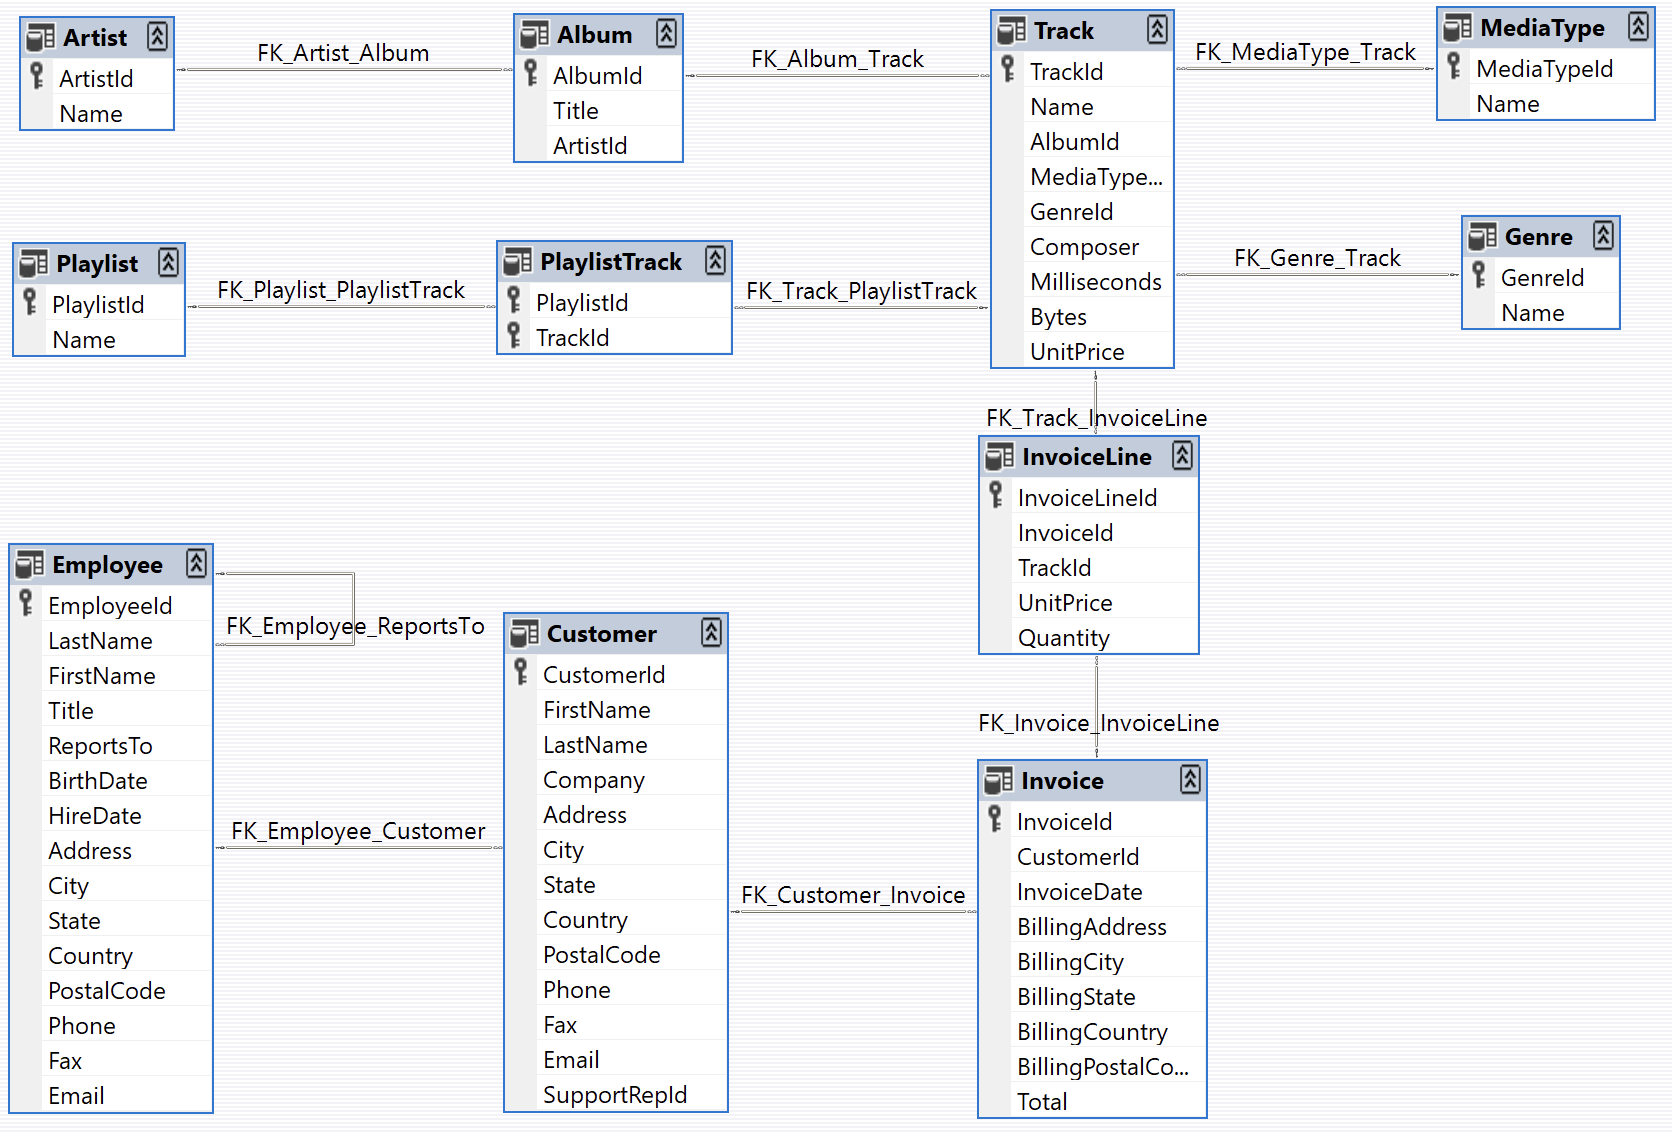
\includegraphics [scale=0.5] {my_folder/images/ex2_schema_ddl}
                  \caption{DDL схемы Chinook в PostgreSQL}
                  \label{fig:ex2_schema_ddl}
                \end{figure}
                \FloatBarrier
          \item Захват изменений и публикация в Kafka \\
                С помощью коннектора Debezium PostgreSQL, настроенного через Kafka Connect, все изменения в таблицах Chinook захватывались из WAL и публиковались в соответствующие топики Kafka(\firef{fig:ex2_kafka_topics}).
                \begin{figure}[h]
                  \center
                  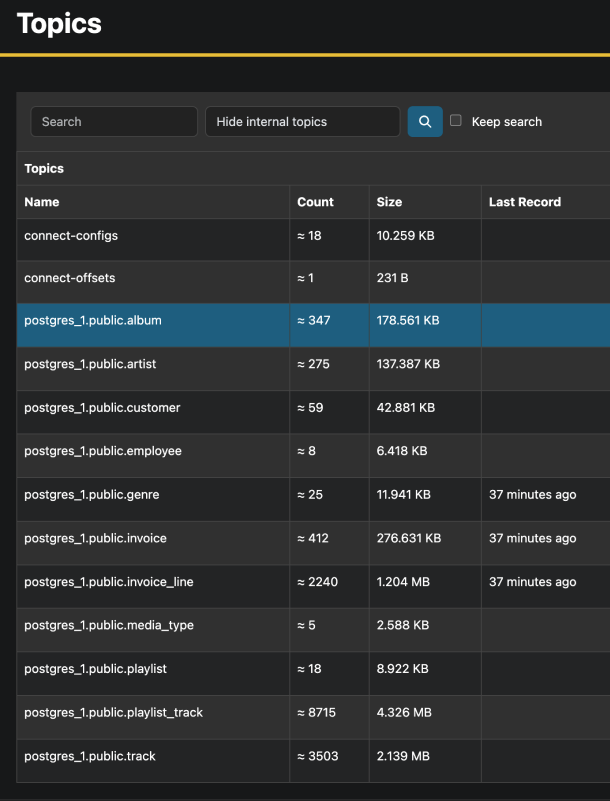
\includegraphics [scale=0.5] {my_folder/images/ex2_kafka_topics}
                  \caption{Список Kafka-топиков в Kafka UI}
                  \label{fig:ex2_kafka_topics}
                \end{figure}
                \FloatBarrier
          \item Архивация данных в S3\\
                Параллельно с основной обработкой, данные из Kafka-топиков архивировались в S3-хранилище (\firef{fig:ex2_s3}). Kafka Connect S3 Sink Connector считывал сообщения из топиков и сохранял их в виде файлов JSON в соответствующие директории внутри S3 бакета. Это обеспечивает долговременное хранение сырых данных.
                \begin{figure}[h]
                  \center
                  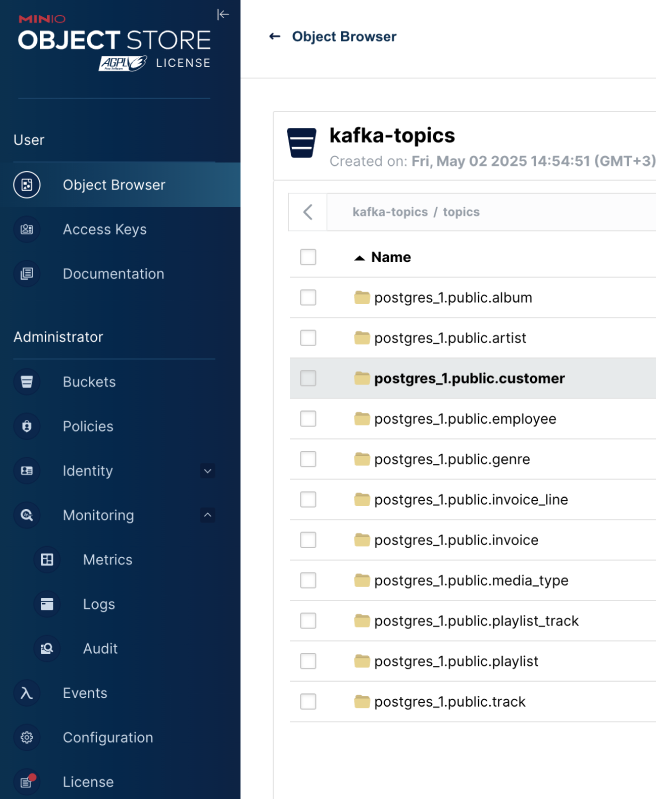
\includegraphics [scale=0.5] {my_folder/images/ex2_s3}
                  \caption{Список директорий в S3, соответствующих топикам Kafka}
                  \label{fig:ex2_s3}
                \end{figure}
                \FloatBarrier
          \item Загрузка и хранение в ClickHouse\\
                Данные о продажах и связанных сущностях доставлялись из Kafka в ClickHouse с использованием стандартного паттерна c предыдущего примера: Kafka Engine таблица для чтения из топика и Materialized View для переноса данных в целевую таблицу на движке MergeTree. Это позволило эффективно хранить данные для аналитических запросов.
          \item Проверка целостности данных \\
                Для подтверждения корректности работы конвейера было выполнено сравнение количества записей в основных таблицах в исходной базе PostgreSQL и в целевых таблицах ClickHouse после завершения загрузки. Результаты сравнения показали идентичное количество строк(\firef{fig:ex2_counts_comparering}).
                \begin{figure}[h]
                  \center
                  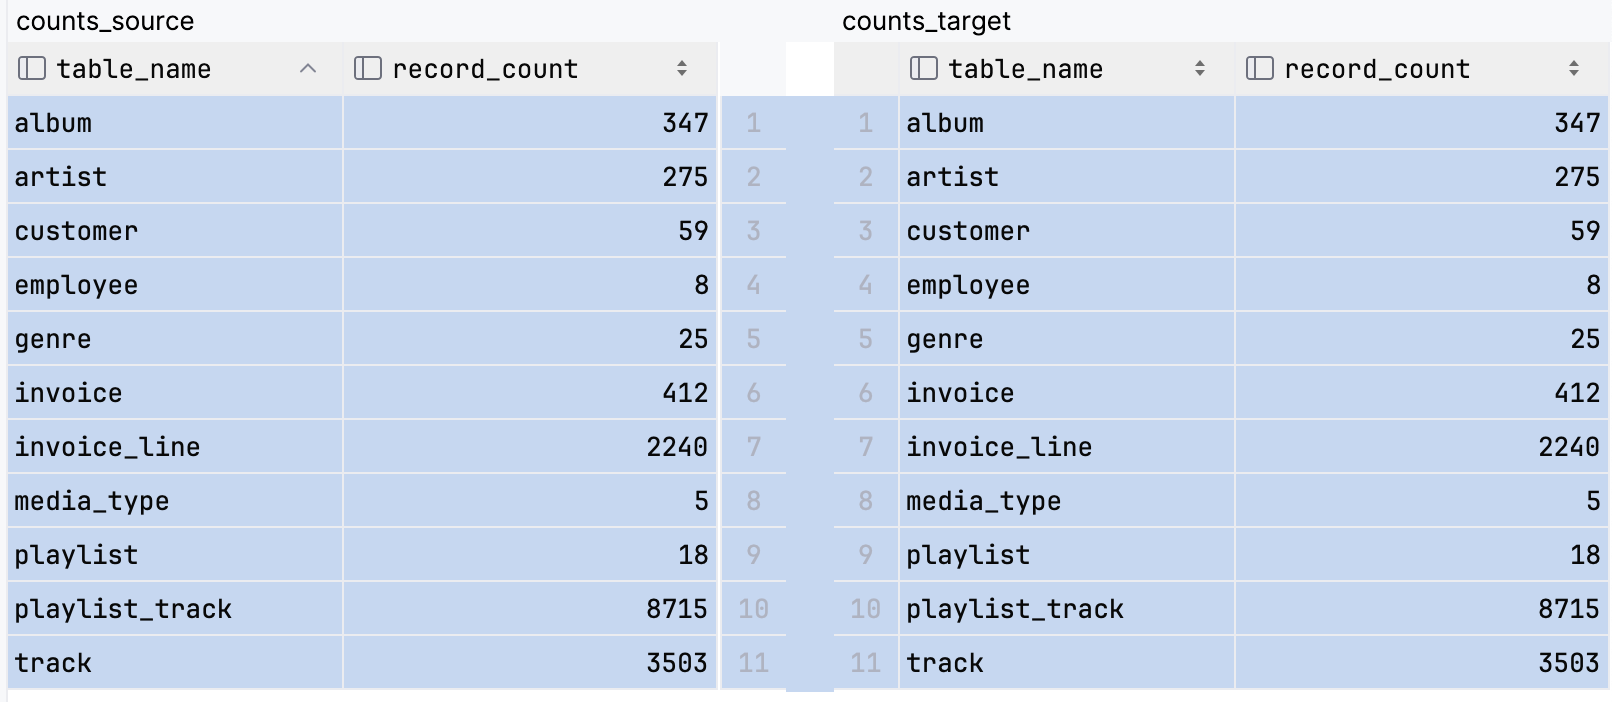
\includegraphics [scale=0.5] {my_folder/images/ex2_counts_comparering}
                  \caption{Сравнение количества строк в PostgreSQL и ClickHouse для Chinook}
                  \label{fig:ex2_counts_comparering}
                \end{figure}
                \FloatBarrier
          \item Анализ и Визуализация (Superset)
                ClickHouse был подключен как источник данных к Superset. На основе данных о продажах (таблица \texttt{invoice\_line}), треках (таблица \texttt{track}) и жанрах (таблица \texttt{genre}), объединенных в ClickHouse, был построен дашборд. Один из ключевых чартов на дашборде отображает количество проданных треков (или сумму продаж) в разрезе музыкальных жанров.
                \begin{figure}[h]
                  \center
                  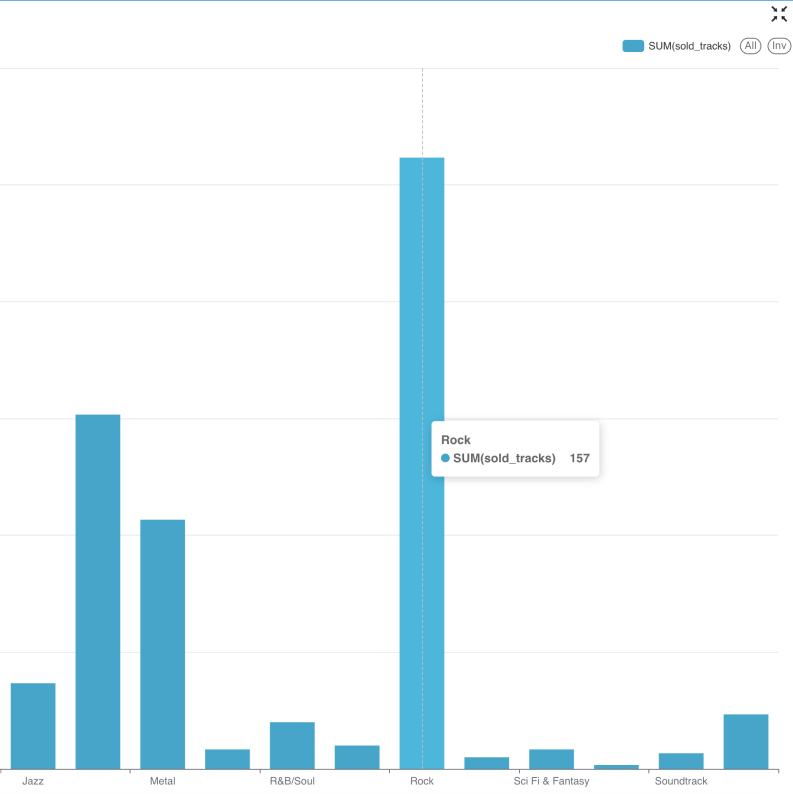
\includegraphics [scale=0.5] {my_folder/images/ex2_superset_chart}
                  \caption{Чарт в Superset "Количество продаж по жанрам"}
                  \label{fig:ex2_superset_chart}
                \end{figure}
                \FloatBarrier
        \end{itemize}
\end{enumerate}

Пример с датасетом Chinook подтверждает гибкость инструмента в развертывании платформ данных для различных сценариев. Была успешно создана инфраструктура и настроен конвейер для сбора, потоковой обработки, архивирования и аналитической обработки данных о музыкальных продажах. Финальная визуализация в Superset демонстрирует готовность платформы к решению реальных бизнес-задач по анализу данных.







% Пример ссылки на литературу \cite{avtonomova:fya,Peskov2004-ru,Kotelnikov2004-ru,Kotelnikov2004}.

%\FloatBarrier % заставить рисунки и другие подвижные (float) элементы остановиться

% \section{Выводы} \label{ch4:conclusion}

% Текст выводов по главе \thechapter.

%% Вспомогательные команды - Additional commands
%
%\newpage % принудительное начало с новой страницы, использовать только в конце раздела
%\clearpage % осуществляется пакетом <<placeins>> в пределах секций
%\newpage\leavevmode\thispagestyle{empty}\newpage % 100 % начало новой страницы           	 % Глава 4
\chapter{Исследование разработанного продукта} \label{ch5}
           	 % Глава 5
\ContinueChapterEnd % завершить размещение глав <<подряд>>
%% Завершение основной части

\chapter*{Заключение} \label{ch-conclusion}
\addcontentsline{toc}{chapter}{Заключение}	% в оглавление 
В рамках настоящей дипломной работы была поставлена и успешно решена актуальная задача автоматизации процесса развертывания и конфигурирования многокомпонентных платформ для работы с большими данными. Актуальность данной задачи обусловлена возрастающей сложностью современных стеков технологий Big Data, требующих значительных временных и экспертных затрат на их первоначальную настройку и последующую поддержку. Ручной процесс конфигурирования подвержен ошибкам, затрудняет воспроизводимость и масштабирование инфраструктуры.

Основной целью работы являлась разработка программного инструмента, способного автоматизировать генерацию конфигураций и артефактов развертывания для типовых компонентов платформ данных на основе декларативного описания.

В ходе выполнения дипломной работы были достигнуты следующие ключевые результаты:

\begin{enumerate}[1.]
    \item Проведен анализ существующих подходов и инструментов для управления конфигурациями и развертывания инфраструктуры, выявлены их преимущества и недостатки применительно к задачам построения платформ больших данных. Это позволило обосновать необходимость разработки специализированного инструмента.
    \item Спроектирован и разработан программный инструмент dpd (Data Platform Deployer). Инструмент использует декларативный подход: пользователь описывает желаемую конфигурацию платформы данных, включая такие компоненты, как PostgreSQL, ClickHouse, Apache Kafka, Kafka Connect с различными коннекторами типа Debezium и S3 Sink, объектное хранилище Minio и систему визуализации Apache Superset, в едином YAML-файле. На основе этого описания dpd автоматически генерирует:
          \begin{itemize}
              \item Файл docker-compose.yml для оркестрации сервисов с корректной настройкой сетевых взаимодействий и передачей параметров между сервисами.
              \item Необходимые конфигурационные файлы для каждого сервиса.
              \item Скрипты инициализации баз данных и других компонентов.
          \end{itemize}
    \item Реализована поддержка расширяемости за счет модульной архитектуры и использования шаблонизатора, что позволяет в будущем добавлять поддержку новых компонентов и кастомизировать генерируемые конфигурации.
    \item Проведено исследование разработанного продукта, ключевым элементом которого стала апробация инструмента dpd в промышленной среде компании ПАО «Магнит». В ходе апробации инструмент использовался для оперативного развертывания тестового стенда с целью тестирования IcebergSinkConnector для Apache Kafka. Результаты апробации, зафиксированные в Акте внедрения (опытной эксплуатации) (Приложение \ref{myappendices::vkr_magnit}), подтвердили практическую применимость и эффективность разработанного решения.
\end{enumerate}
Все положения, выносимые на защиту, были подтверждены в ходе исследования:

\begin{itemize}
    \item Автоматическая генерация конфигураций элементов инфраструктуры программных систем для работы с большими данными: продемонстрирована способность dpd генерировать полный набор корректных артефактов на основе декларативного описания, что было подтверждено в ходе апробации.
    \item Значительное снижение трудоемкости и времени развертывания комплексной платформы данных: экспертная оценка специалистов ПАО «Магнит» показала, что использование dpd существенно сокращает время и усилия, необходимые для подготовки инфраструктуры, по сравнению с ручным подходом.
    \item Обеспечение корректности, согласованности и воспроизводимости конфигурации взаимосвязанных компонентов платформы данных: практическое применение dpd показало, что сгенерированные конфигурации обеспечивают корректное взаимодействие всех компонентов "из коробки"\,, а сам процесс развертывания становится полностью воспроизводимым.
\end{itemize}
Практическая значимость работы заключается в создании инструмента, который упрощает и ускоряет процесс развертывания платформ больших данных, снижает порог входа для инженеров, уменьшает количество ошибок, связанных с человеческим фактором, и способствует стандартизации конфигураций. Это особенно ценно в условиях динамично развивающихся проектов и при необходимости частого создания тестовых или демонстрационных окружений.


Разработанный инструмент dpd обладает потенциалом для дальнейшего развития, включая:
\begin{itemize}
    \item Расширение списка поддерживаемых компонентов и облачных сервисов.
    \item Интеграцию с системами CI/CD для полной автоматизации жизненного цикла инфраструктуры.
    \item Разработку графического пользовательского интерфейса для упрощения описания конфигураций.
    \item Более глубокую кастомизацию генерируемых скриптов и конфигураций.
\end{itemize}

Таким образом, цели, поставленные в дипломной работе, были полностью достигнуты. Разработанный программный инструмент dpd представляет собой законченное решение, обладающее как теоретической новизной в части подхода к автоматической генерации конфигураций на основе формализованной модели, так и высокой практической ценностью, подтвержденной результатами апробации в реальных условиях.



% Заключение (2 -- 5 страниц) обязательно содержит выводы по теме работы, \textit{конкретные
% предложения и рекомендации} по исследуемым вопросам. Количество общих выводов
% должно вытекать из количества задач, сформулированных во введении выпускной
% квалификационной работы.

% Предложения и рекомендации должны быть органически увязаны с выводами
% и направлены на улучшение функционирования исследуемого объекта. При разработке
% предложений и рекомендаций обращается внимание на их обоснованность,
% реальность и практическую приемлемость.

% Заключение не должно содержать новой информации, положений, выводов и
% т. д., которые до этого не рассматривались в выпускной квалификационной работе.
% Рекомендуется писать заключение в виде тезисов.

% Последним абзацем в заключении можно выразить благодарность всем людям, которые помогали автору в написании ВКР.        	 % Заключение

%% Наличие следующих перечней не исключает расшифровку сокращения и условного обозначения при первом упоминании в тексте!
% % \chapter*{Список сокращений и условных обозначений}             % Заголовок
% \addcontentsline{toc}{chapter}{Список сокращений и условных обозначений}  % Добавляем его в оглавление
% \noindent
% \addtocounter{table}{-1}% Нужно откатить на единицу счетчик номеров таблиц, так как следующая таблица сделана для удобства представления информации по ГОСТ
% %\begin{longtabu} to \dimexpr \textwidth-5\tabcolsep {r X}
% \begin{longtabu} to \textwidth {r X} % Таблицу не прорисовываем!
% % Жирное начертание для математических символов может иметь
% % дополнительный смысл, поэтому они приводятся как в тексте
% % диссертации
% \textbf{DOI} & Digital Object Identifier. \\
% \textbf{WoS} & Web of Science. \\
% \textbf{ВКР}  & Выпускная квалификационная работа. \\
% \textbf{ТГ-объект}  & Текстово-графический объект. \\
% %$\begin{rcases}
% %a_n\\
% %b_n
% %\end{rcases}$  & 
% %\begin{minipage}{\linewidth}
% %Коэффициенты разложения Ми в дальнем поле, соответствующие
% %электрическим и магнитным мультиполям.
% %\end{minipage}
% %\\
% %${\boldsymbol{\hat{\mathrm e}}}$ & Единичный вектор. \\
% %$E_0$ & Амплитуда падающего поля.\\
% %$\begin{rcases}
% %a_n\\
% %b_n
% %\end{rcases}$  & 
% %Коэффициенты разложения Ми в дальнем поле соответствующие
% %электрическим и магнитным мультиполям ещё раз, но без окружения
% %minipage нет вертикального выравнивания по центру.
% %\\
% %$j$ & Тип функции Бесселя.\\
% %$k$ & Волновой вектор падающей волны.\\
% %
% %$\begin{rcases}
% %a_n\\
% %b_n
% %\end{rcases}$  & 
% %\begin{minipage}{\linewidth}
% %\vspace{0.7em}
% %Коэффициенты разложения Ми в дальнем поле соответствующие
% %электрическим и магнитным мультиполям, теперь окружение minipage есть
% %и добавленно много текста, так что описание группы условных
% %обозначений значительно превысило высоту этой группы... Для отбивки
% %пришлось добавить дополнительные отступы.
% %\vspace{0.5em}
% %\end{minipage}
% %\\
% %$L$ & Общее число слоёв.\\
% %$l$ & Номер слоя внутри стратифицированной сферы.\\
% %$\lambda$ & Длина волны электромагнитного излучения
% %в вакууме.\\
% %$n$ & Порядок мультиполя.\\
% %$\begin{rcases}
% %{\mathbf{N}}_{e1n}^{(j)}&{\mathbf{N}}_{o1n}^{(j)}\\
% %{\mathbf{M}_{o1n}^{(j)}}&{\mathbf{M}_{e1n}^{(j)}}
% %\end{rcases}$  & Сферические векторные гармоники.\\
% %$\mu$  & Магнитная проницаемость в вакууме.\\
% %$r,\theta,\phi$ & Полярные координаты.\\
% %$\omega$ & Частота падающей волны.\\
% %
% %  \textbf{BEM} & Boundary element method, метод граничных элементов.\\
% %  \textbf{CST MWS} & Computer Simulation Technology Microwave Studio.
% \end{longtabu}
		         % Необязательная рубрика! Список сокращений и условных обозначений

\chapter*{Словарь терминов}             % Заголовок
\addcontentsline{toc}{chapter}{Словарь терминов}  % Добавляем его в оглавление

\textbf{API (Application Programming Interface)} --- интерфейс программирования приложений; набор готовых классов, процедур, функций, структур и констант, предоставляемых приложением (библиотекой, сервисом) для использования во внешних программных продуктах.

\textbf{ANTLR (ANother Tool for Language Recognition)} --- генератор парсеров, который используется для создания компиляторов, интерпретаторов и других инструментов, работающих с языками программирования или формальными языками.

\textbf{Apache Kafka} --- распределённая платформа для обработки потоковых данных, используемая для построения конвейеров данных реального времени и потоковых приложений.

\textbf{Apache Superset} --- веб-приложение с открытым исходным кодом для исследования и визуализации данных.

\textbf{Arenadata} --- российская компания, разрабатывающая платформу для сбора, хранения и обработки больших данных на основе технологий с открытым исходным кодом.

\textbf{Docker} --- программная платформа для быстрой разработки, тестирования и развертывания приложений. Docker упаковывает программное обеспечение в стандартизированные блоки, называемые контейнерами, которые включают все необходимое для работы: библиотеки, системные инструменты, код и среду выполнения.

\textbf{Docker Compose} --- инструмент для определения и запуска многоконтейнерных приложений Docker. С помощью Compose используется YAML-файл для настройки служб приложения.

\textbf{DSL (Domain-Specific Language)} --- язык, специализированный для конкретной области применения. В контексте работы, это язык описания конфигурации платформы данных.

\textbf{ETL (Extract, Transform, Load)} --- извлечение, преобразование, загрузка; один из основных процессов в управлении хранилищами данных, который включает извлечение данных из внешних источников, их преобразование и очистку для соответствия нуждам бизнес-модели и загрузку в хранилище данных.

\textbf{IaC (Infrastructure as Code)} --- инфраструктура как код; подход к управлению и предоставлению компьютерных центров обработки данных через машиночитаемые файлы определений, а не через физическую конфигурацию оборудования или интерактивные инструменты настройки.

\textbf{JSON (JavaScript Object Notation)} --- текстовый формат обмена данными, основанный на JavaScript. Легко читаем людьми и легко обрабатывается компьютерами.

\textbf{Kafka Connect} --- фреймворк для надежной потоковой передачи данных между Apache Kafka и другими системами. Используется для создания коннекторов, которые перемещают большие наборы данных в Kafka и из Kafka.

\textbf{Minio} --- высокопроизводительное распределенное объектное хранилище, совместимое с Amazon S3 API.

\textbf{PostgreSQL} --- свободная объектно-реляционная система управления базами данных (СУБД).

\textbf{S3 (Simple Storage Service)} --- сервис простого хранения данных, изначально разработанный Amazon Web Services; стандарт де-факто для API объектных хранилищ.

\textbf{SQL (Structured Query Language)} --- язык структурированных запросов; декларативный язык программирования, применяемый для создания, модификации и управления данными в реляционной базе данных.

\textbf{Yandex Cloud} --- облачная платформа, предоставляемая компанией Яндекс, включающая различные сервисы, в том числе для работы с большими данными.

\textbf{YAML (YAML Ain't Markup Language)} --- рекурсивный акроним, «YAML — не язык разметки»; дружественный к человеку формат сериализации данных, часто используемый для конфигурационных файлов.

\textbf{Аналитика данных (Data Analytics)} --- процесс инспектирования, очистки, преобразования и моделирования данных с целью извлечения полезной информации, формирования выводов и поддержки принятия решений.

\textbf{Большие данные (Big Data)} --- совокупность подходов, инструментов и методов обработки структурированных и неструктурированных данных огромных объёмов и значительного многообразия для получения воспринимаемых человеком результатов.

\textbf{Брокер сообщений (Message Broker)} --- промежуточное программное обеспечение, которое преобразует сообщения из формального протокола обмена сообщениями отправителя в формальный протокол обмена сообщениями получателя.

\textbf{Визуализация данных (Data Visualization)} --- представление данных в графическом формате для облегчения их восприятия и анализа.

\textbf{Генератор конфигураций (Configuration Generator)} --- программный инструмент, который автоматически создает конфигурационные файлы для одной или нескольких систем на основе входных параметров или шаблонов.

\textbf{Декларативное описание (Declarative Description)} --- способ описания системы или процесса, при котором указывается *что* должно быть достигнуто, а не *как* это сделать.

\textbf{Интегрированная платформа данных (Integrated Data Platform)} --- комплексное решение, объединяющее различные инструменты и сервисы для сбора, хранения, обработки и анализа данных в единой среде.

\textbf{Инфраструктура (Infrastructure)} --- совокупность взаимосвязанных обслуживающих структур или объектов, составляющих и/или обеспечивающих основу функционирования системы. В ИТ это физическое и виртуальное оборудование, сети, операционные системы, хранилища данных.

\textbf{Коннектор (Connector)} --- в Kafka Connect, компонент, отвечающий за интеграцию с конкретным источником или приемником данных.

\textbf{Контейнеризация (Containerization)} --- метод виртуализации на уровне операционной системы, при котором приложения запускаются в изолированных пространствах, называемых контейнерами.

\textbf{Конфигурационный файл (Configuration File)} --- файл, используемый для настройки параметров компьютерной программы или операционной системы.

\textbf{Метаданные (Metadata)} --- данные о данных; информация, описывающая свойства других данных.

\textbf{Метамодель (Metamodel)} --- модель, описывающая структуру или правила построения других моделей.

\textbf{Облачные вычисления (Cloud Computing)} --- модель обеспечения повсеместного и удобного сетевого доступа по требованию к общему пулу конфигурируемых вычислительных ресурсов (например, сетям передачи данных, серверам, устройствам хранения данных, приложениям и сервисам), которые могут быть оперативно предоставлены и освобождены с минимальными усилиями по управлению и необходимостью взаимодействия с провайдером.

\textbf{Объектное хранилище (Object Storage)} --- архитектура хранения данных, которая управляет данными как объектами, в отличие от других архитектур хранения, таких как файловые системы, которые управляют данными как иерархией файлов, и блочные хранилища, которые управляют данными как блоками внутри секторов и дорожек.

\textbf{Оркестрация контейнеров (Container Orchestration)} --- автоматизация развертывания, масштабирования и управления контейнеризированными приложениями.

\textbf{Парсер (Parser)} --- часть компилятора или интерпретатора, отвечающая за синтаксический анализ входной последовательности символов (например, исходного кода) с целью построения структуры данных, обычно дерева разбора или абстрактного синтаксического дерева.

\textbf{Платформа данных (Data Platform)} --- интегрированный набор технологий, используемых для сбора, хранения, обработки, анализа и управления данными.

\textbf{Потоковая обработка данных (Stream Processing)} --- парадигма обработки данных, при которой данные обрабатываются непрерывно по мере их поступления, а не пакетами.

\textbf{Развертывание (Deployment)} --- процесс установки, настройки и активации программного обеспечения или инфраструктуры в целевой среде, делая его доступным для использования.

\textbf{Репозиторий (Repository)} --- место, где хранятся и поддерживаются какие-либо данные. Часто используется в контексте систем управления версиями (например, Git-репозиторий).

\textbf{Скрипт (Script)} --- программа или последовательность инструкций, которая автоматизирует выполнение задач.

\textbf{СУБД (Система Управления Базами Данных)} --- совокупность программных и языковых средств, предназначенных для создания, ведения и совместного использования баз данных многими пользователями.

\textbf{Топик (Topic)} --- в Apache Kafka, именованная категория или канал, в который продюсеры публикуют сообщения и из которого консьюмеры читают сообщения.

\textbf{Управляемый сервис (Managed Service)} --- сервис, предоставляемый облачным провайдером, который берет на себя задачи по управлению, обслуживанию и масштабированию базовой инфраструктуры этого сервиса.

\textbf{Хранилище данных (Data Warehouse)} --- предметно-ориентированная, интегрированная, привязанная ко времени и неизменяемая совокупность данных, предназначенная для поддержки принятия управленческих решений.

\textbf{CDC (Change Data Capture)} --- захват изменений данных; процесс отслеживания изменений в источнике данных (например, базе данных) и доставки этих изменений в другие системы или хранилища.

\textbf{ClickHouse} --- быстрая аналитическая СУБД с открытым исходным кодом, работающая на основе столбцового хранения данных.

\textbf{dpd (Data Platform Deployer)} --- разрабатываемый инструмент для автоматической генерации конфигураций и развертывания платформы данных.
    		 % Необязательная рубрика! Словарь терминов
% По порядку после Списка сокращений и условных обозначений, если есть.	


\input{my_folder/references}		     % Список литературы

% Здесь можно поместить список иллюстративного материала

\appendix % не редактировать / keep unmodified


\chapter{Грамматика языка DPD}\label{grammatic-dpd}							% Заголовок
%\addcontentsline{toc}{chapter}{Second call for chapters to participate in the book Machine learning in analysis of biomedical and socio-economic data}	% Добавляем его в оглавление
\begin{longtable}{|p{3in}|p{3in}|}
    \caption{Грамматика языка DPD в форме ANTLR}\\
    \hline
    Грамматика ANTLR4            & Комментарий                                                                                                                                                           \\ \hline
    \begin{minipage}{2.6in}
        \begin{verbatim}
grammar ConfigDSL;
        \end{verbatim}
    \end{minipage}      &                                                                                                                                                                               \\ \hline
    \begin{minipage}{3in}
        \begin{verbatim}
configFile
: projectDef
sourcesDef
streamingDef
storageDef
biDef EOF
;
\end{verbatim}
    \end{minipage}        &
    \begin{minipage}{3in}Корневое правило: определяет общую структуру конфигурационного файла, состоящего из последовательных блоков\end{minipage}                                                       \\ \hline
    \begin{minipage}{2.6in}
        \begin{verbatim}
projectDef
: PROJECT COLON NAME COLON 
STRING VERSION COLON STRING 
DESCRIPTION COLON STRING
;
    \end{verbatim}
    \end{minipage} &
    \begin{minipage}{3in}Правило для секции "project": описывает метаданные проекта\end{minipage}                                                                                                        \\ \hline
    \begin{minipage}{3in}
        \begin{verbatim}
sourcesDef
: SOURCES COLON 
sourceItem+
        ;
    \end{verbatim}
    \end{minipage}
                                 &
    \begin{minipage}{2.6in}
        Правило для секции «sources»: определяет список источников данных.
    \end{minipage}
    \\ \hline

    \begin{minipage}{3in}
        \begin{verbatim}
sourceItem
: DASH NAME COLON STRING 
TYPE COLON sourceType
( PORT COLON NUMBER )?
( USERNAME COLON STRING )?
( PASSWORD COLON STRING )?
( ACCESS_KEY COLON STRING )?
( SECRET_KEY COLON STRING )?
( REGION COLON STRING )?
( BUCKET COLON STRING )?
;
    \end{verbatim}
    \end{minipage}
                                 &
    \begin{minipage}{2.6in}
        Правило для описания одного источника данных: имя, тип (Postgres/S3) и опциональные параметры (порт, учётные данные, детали S3).
    \end{minipage}
    \\ \hline

    \begin{minipage}{3in}
        \begin{verbatim}
sourceType
: POSTGRES
| S3
;
    \end{verbatim}
    \end{minipage}
                                 &
    \begin{minipage}{2.6in}
        Правило для определения типа источника данных (PostgreSQL или S3).
    \end{minipage}
    \\ \hline

    \begin{minipage}{3in}
        \begin{verbatim}
streamingDef
: STREAMING COLON 
(kafkaDef | connectDef)+
        ;
    \end{verbatim}
    \end{minipage}
                                 &
    \begin{minipage}{2.6in}
        Правило для секции «streaming»: задаёт компоненты потоковой обработки (Kafka или Kafka Connect).
    \end{minipage}
    \\ \hline

    \begin{minipage}{3in}
        \begin{verbatim}
kafkaDef
: KAFKA COLON 
NUM_BROKERS COLON 
NUMBER
;
    \end{verbatim}
    \end{minipage}
                                 &
    \begin{minipage}{2.6in}
        Правило для конфигурации Kafka: число брокеров.
    \end{minipage}
    \\ \hline

    \begin{minipage}{3in}
        \begin{verbatim}
connectDef
: CONNECT COLON 
NAME COLON STRING
        ;
    \end{verbatim}
    \end{minipage}
                                 &
    \begin{minipage}{2.6in}
        Правило для конфигурации Kafka Connect: имя инстанса.
    \end{minipage}
    \\ \hline

    \begin{minipage}{3in}
        \begin{verbatim}
storageDef
: STORAGE COLON 
clickhouseDef
;

clickhouseDef
: CLICKHOUSE COLON 
NAME COLON STRING
;
    \end{verbatim}
    \end{minipage}
                                 &
    \begin{minipage}{2.6in}
        Правило для секции «storage»: задаёт компонент хранения данных и его параметры (ClickHouse).
    \end{minipage}
    \\ \hline

    \begin{minipage}{3in}
        \begin{verbatim}
biDef
: BI COLON supersetDef
;

supersetDef
: SUPERSET COLON 
NAME COLON STRING
( USERNAME COLON STRING )?
( PASSWORD COLON STRING )?
;
    \end{verbatim}
    \end{minipage}
                                 &
    \begin{minipage}{2.6in}
        Правило для секции «bi»: задаёт инструмент BI (Apache Superset) и его опциональные параметры.
    \end{minipage}
    \\ \hline

    \begin{minipage}{3in}
        \begin{verbatim}
PROJECT     : 'project';
SOURCES     : 'sources';
STREAMING   : 'streaming';
STORAGE     : 'storage';
BI          : 'bi';
KAFKA       : 'kafka';
CONNECT     : 'connect';
CLICKHOUSE  : 'clickhouse';
SUPERSET    : 'superset';
NAME        : 'name';
VERSION     : 'version';
DESCRIPTION : 'description';
TYPE        : 'type';
PORT        : 'port';
USERNAME    : 'username';
PASSWORD    : 'password';
ACCESS_KEY  : 'access_key';
SECRET_KEY  : 'secret_key';
REGION      : 'region';
BUCKET      : 'bucket';
NUM_BROKERS : 'num_brokers';
POSTGRES    : 'postgres';
S3          : 's3';
COLON       : ':';
DASH        : '-';
STRING      : 
'"' ( ~[\\"] | '\\' . )*? '"' ;
NUMBER      : [0-9]+ ;
WS          : 
[ \t\r\n]+ -> skip ;
    \end{verbatim}
    \end{minipage}
                                 &
    \begin{minipage}{2.6in}
        Лексемы: ключевые слова, разделители, строковые и числовые литералы, пробельные символы.                                                                                     \end{minipage} \\ \hline
\end{longtable}
% В SPbPU-BCI-template {\itshape автоматически выставляются необходимые настройки и в исходном тексте шаблона приведены примеры оформления текстово-графических объектов}, поэтому авторам достаточно заполнить имеющийся шаблон текстом главы (статьи), не вдаваясь в детали оформления, описанные далее. Возможный <<быстрый старт>> оформления главы (статьи) под Windows следующий\footnote{Внимание! Пример оформления подстрочной ссылки (сноски).}:

% \begin{enumerate}
% 	\item Установка полной версии TeX Live  \cite{latex-texlive}.  В процессе установки лучше выставить параметр доустановки пакетов <<на лету>>.
	
% 	\item Установка TexStudio \cite{latex-texstudio}.
	
% %		\item установка шрифтов PSCyr для работы с TimesNew\-Roman\-PSMT  	\href{https://github.com/AndreyAkinshin/Russian-Phd-LaTeX-Dissertation-Template/blob/master/PSCyr/Windows.md}{по данной инструкции}. В итоговом документе будет, скорее всего, использован Newton.
	
% %	\item Переименование следующих файлов, где вместо \texttt{AuthorsSur\-names} необходимо подставить фамилии авторов (можно сокращать до первых четырех букв): 
% %	
% %	\begin{enumerate}
% %		\item Основной файл \texttt{Book\_title\_ch\_Authors\-Sur\-names.tex}.
% %		\item Библиография \texttt{biblio\textbackslash{}Book\_title\_bib\_Authors\-Sur\-na\-mes\-.bib}.
% %		\item Пользовательские настройки (при необходимости), \texttt{common\textbackslash{}Book\_\-tit\-le\_ext\_Authors\-Sur\-names.tex}. 
% %	\end{enumerate}
% %	
% %	\item После открытия основного файла \texttt{Book\_title\_ch\_Authors\-Sur\-names.tex} (с новым названием)   переименовать названия по аналогии в следующих командах \texttt{\textbackslash{}input\{\}}:
% %	
% %	\begin{enumerate}
% %		\item \texttt{biblio/Book\_title\_bib\_Authors\-Sur\-names.bib},
% %		\item \texttt{common/Book\_title\_ext\_Authors\-Sur\-names.tex (при необходимости) }.
% %	\end{enumerate}
% %	
	
% 	\item Запуск TexStudio и компиляция \verb|my_chapter.tex| с помощью команды <<Build\&View>> (например, с помощью двойной зелёной стрелки в верхней панели). {\itshape Иногда, для достижения нужного результата необходимо несколько раз скомпилировать документ.}
	
% 	\item В случае, если не отобразилась библиография, можно
	
% 	\begin{itemize}
% 		\item воспользоваться командой Tools $\to$ Commands $\to$ Biber, затем запустив Build\&View;
		
% 		\item настроить автоматическое включение библиографии в настройках Options $\to$ Configure TexStudio $\to$ Build $\to$  Build\&View (оставить по умолчанию, если сборка происходит слишком долго): \texttt{txs:///pdflatex | txs:///biber | txs:///pdflatex | txs:///pdflatex | txs:///\-view-pdf}.
% 	\end{itemize}
	
% \end{enumerate}

% В случае возникновения ошибок, попробуйте скомпилировать документ до последних действий или внимательно ознакомьтесь с описанием проблемы в log-файле. Бывает полезным переход (по подсказке TexStudio) в нужную строку в pdf-файле или запрос с текстом ошибке в поисковиках. Наиболее вероятной проблемой при первой компиляции может быть отсутствие какого-либо установленного пакета \LaTeX. 

% В случае корректной работы настройки <<установка на лету>> все дополнительные пакеты будут скачиваться и устанавливаться в автоматическом режиме. Если доустановка пакетов осуществляется медленно (несколько пакетов за один запуск компилятора), то можно попробовать установить их в ручном режиме следующим образом:

% \begin{enumerate}[1.]
% 	\item Запустите программу: меню $\to$ все программы $\to$ MikTeX $\to$ Maintenance (Admin) $\to$ MiKTeX Package Manager (Admin).
% 	\item Пользуясь поиском, убедитесь, что нужный пакет присутствует, но не установлен (если пакет отсутствует воспользуйтесь сначала MiKTeX Update (Admin)).
% 	\item Выделив строку с пакетом (возможно выбрать несколько или вообще все неустановленные пакеты), выполните установку Tools $\to$ Install или с помощью контекстного меню.
% 	\item После завершения установки запустите программу MiKTeX Settings (Admin).
% 	\item Обновите базу данных имен файлов Refresh FNDB.
% \end{enumerate}


% Для проверки текста статьи на русском языке полезно также воспользоваться настройками Options $\to$ Configure TexStudio $\to$ Language Checking $\to$  Default Language. Если русский язык <<ru\_RU>> не будет доступен в меню выбора, то необходимо вначале выполнить Import Dictionary, скачав из интернета любой русскоязычный словарь. 


% %\chapter{\normalfont\normalsize{}Часто задаваемые вопросы (FAQ)}\label{Appendix-FAQ}							% Заголовок
% %%\addcontentsline{toc}{chapter}{Second call for chapters to participate in the book Machine learning in analysis of biomedical and socio-economic data}	% Добавляем его в оглавление


% Далее приведены формулы \eqref{eq:Pi-app2}, \eqref{eq:Pi-app2-},  \firef{fig:spbpu_hydrotower-app2}, \firef{fig:spbpu_hydrotower-app2-}, \taref{tab:ToyCompare-app2}, \taref{tab:ToyCompare-app2-}.


% \begin{equation}% лучше не оставлять пропущенную строку (\par) перед окружениями для избежания лишних отсупов в pdf
% \label{eq:Pi-app2-} % eq - equations, далее название, ch поставлено для избежания дублирования
% \pi \approx 3,141.
% \end{equation}

% %
% \begin{figure}[ht!] 
% 	\center
% 	\includegraphics [scale=0.27] {my_folder/images//spbpu_hydrotower}
% 	\caption{Вид на гидробашню СПбПУ \cite{spbpu-gallery}} 
% 	\label{fig:spbpu_hydrotower-app2-}  
% \end{figure}

% \begin{table} [htbp]% Пример оформления таблицы
% 	\centering\small
% 	\caption{Представление данных для сквозного примера по ВКР \cite{Peskov2004}}%
% 	\label{tab:ToyCompare-app2-}		
% 	\begin{tabular}{|l|l|l|l|l|l|}
% 		\hline
% 		$G$&$m_1$&$m_2$&$m_3$&$m_4$&$K$\\
% 		\hline
% 		$g_1$&0&1&1&0&1\\ \hline
% 		$g_2$&1&2&0&1&1\\ \hline
% 		$g_3$&0&1&0&1&1\\ \hline
% 		$g_4$&1&2&1&0&2\\ \hline
% 		$g_5$&1&1&0&1&2\\ \hline
% 		$g_6$&1&1&1&2&2\\ \hline		
% 	\end{tabular}	
% 	\normalsize% возвращаем шрифт к нормальному
% \end{table}




% \section{Параграф приложения}\label{app-2-1}							


% \subsection{Название подпараграфа} \label{ch2:subsec-title-abbr} %название по-русски


% Название подпараграфа оформляется с помощью команды  \texttt{\textbackslash{}subsection\{...\}}.

% Использование подподпараграфов в основной части крайне не рекомендуется.
% \subsubsection{Название подподпараграфа}\label{ch2:subsubsec-title-abbr} %название по-русски

% \begin{equation}% лучше не оставлять пропущенную строку (\par) перед окружениями для избежания лишних отсупов в pdf
% \label{eq:Pi-app2} % eq - equations, далее название, ch поставлено для избежания дублирования
% \pi \approx 3,141.
% \end{equation}
% %
% %
% \begin{figure}[ht!] 
% 	\center
% 	\includegraphics [scale=0.27] {my_folder/images//spbpu_hydrotower}
% 	\caption{Вид на гидробашню СПбПУ \cite{spbpu-gallery}} 
% 	\label{fig:spbpu_hydrotower-app2}  
% \end{figure}
% %




% \begin{table}[t!]% Пример оформления таблицы
% 	\centering\small
% 	\caption{Представление данных для сквозного примера по ВКР \cite{Peskov2004}}%
% 	\label{tab:ToyCompare-app2}		
% 	\begin{tabular}{|l|l|l|l|l|l|}
% 		\hline
% 		$G$&$m_1$&$m_2$&$m_3$&$m_4$&$K$\\
% 		\hline
% 		$g_1$&0&1&1&0&1\\ \hline
% 		$g_2$&1&2&0&1&1\\ \hline
% 		$g_3$&0&1&0&1&1\\ \hline
% 		$g_4$&1&2&1&0&2\\ \hline
% 		$g_5$&1&1&0&1&2\\ \hline
% 		$g_6$&1&1&1&2&2\\ \hline		
% 	\end{tabular}	
% 	\normalsize% возвращаем шрифт к нормальному
% \end{table}


%% В случае, когда таблица (рисунок) размещаются на последней странице, для переноса названия приложения на новую строку используем:
\NewPage % начать новое приложение с новой страницы 			     % Приложение 1

\chapter{SQL код для забора данных из Kafka в ClickHouse}\label{ex_1_sql}							% 

В приложениии приведен SQL код для забора данных из Kafka топика в ClickHouse для таблицы \texttt{orders}

\begin{lstlisting}[%
	language=SQL,%      язык
	numbers=left,%      нумерация строк слева
	stepnumber=1,%      номер каждой строки
	firstnumber=1,%     начинают с 1
	numberstyle=\tiny\color{gray},% стиль номеров
	numbersep=5pt,%     отступ номеров от кода
	basicstyle=\ttfamily\small,% шрифт кода
	keywordstyle=\color{blue}\bfseries,% стиль ключевых слов
	stringstyle=\color{red},% стиль строковых литералов
	commentstyle=\color{green!50!black},% стиль комментариев
	frame=single,%      рамка вокруг кода
	breaklines=true,%   автоматический перенос строк
	caption={SQL код для забора данных из Kafka в ClickHouse},%
	label={lst:clickhouse_schema}% метка для ссылки
  ]
  CREATE TABLE clickhouse_1_db.kafka_orders (data String)
  ENGINE = Kafka()
  SETTINGS kafka_broker_list = 'kafka-0:9092,kafka-1:9092,kafka-2:9092,kafka-3:9092,kafka-4:9092,kafka-5:9092',
		   kafka_topic_list  = 'postgres_1.public.orders',
		   kafka_group_name  = 'kafka-ch',
		   kafka_format      = 'JSONAsString';
  
  CREATE TABLE clickhouse_1_db.orders
  (
	 order_id            Int16,
	 customer_id         Nullable(String),
	 employee_id         Nullable(Int16),
	 order_date          Nullable(Date),
	 required_date       Nullable(Date),
	 shipped_date        Nullable(Date),
	 ship_via            Nullable(Int16),
	 freight             Nullable(Float32),
	 ship_name           Nullable(String),
	 ship_address        Nullable(String),
	 ship_city           Nullable(String),
	 ship_region         Nullable(String),
	 ship_postal_code    Nullable(String),
	 ship_country        Nullable(String)
  )
  ENGINE = MergeTree()
  ORDER BY order_id;
  
  CREATE MATERIALIZED VIEW clickhouse_1_db.kafka_orders_mv
  TO clickhouse_1_db.orders AS
  SELECT
	 CAST(JSON_VALUE(data, '$.after.order_id')              AS Int16)           AS order_id,
	 CAST(JSON_VALUE(data, '$.after.customer_id')           AS Nullable(String)) AS customer_id,
	 CAST(JSON_VALUE(data, '$.after.employee_id')           AS Nullable(Int16))  AS employee_id,
	 CAST(toDate(CAST(JSON_VALUE(data, '$.after.order_date')    AS Nullable(Int64))) AS Nullable(Date))   AS order_date,
	 CAST(toDate(CAST(JSON_VALUE(data, '$.after.required_date') AS Nullable(Int64))) AS Nullable(Date))   AS required_date,
	 CAST(toDate(CAST(JSON_VALUE(data, '$.after.shipped_date')  AS Nullable(Int64))) AS Nullable(Date))   AS shipped_date,
	 CAST(JSON_VALUE(data, '$.after.ship_via')              AS Nullable(Int16))  AS ship_via,
	 CAST(JSON_VALUE(data, '$.after.freight')               AS Nullable(Float32))AS freight,
	 CAST(JSON_VALUE(data, '$.after.ship_name')             AS Nullable(String)) AS ship_name,
	 CAST(JSON_VALUE(data, '$.after.ship_address')          AS Nullable(String)) AS ship_address,
	 CAST(JSON_VALUE(data, '$.after.ship_city')             AS Nullable(String)) AS ship_city,
	 CAST(JSON_VALUE(data, '$.after.ship_region')           AS Nullable(String)) AS ship_region,
	 CAST(JSON_VALUE(data, '$.after.ship_postal_code')      AS Nullable(String)) AS ship_postal_code,
	 CAST(JSON_VALUE(data, '$.after.ship_country')          AS Nullable(String)) AS ship_country
  FROM clickhouse_1_db.kafka_orders;
  \end{lstlisting}

% В приложении приведены формулы \eqref{eq:Pi-app}, \eqref{eq:Pi-app-}, \firef{fig:spbpu_hydrotower-app}, \firef{fig:spbpu_hydrotower-app-}, \taref{tab:ToyCompare-app}, \taref{tab:ToyCompare-app-}\footnote{Внимание! Пример оформления подстрочной ссылки (сноски).}.


% \begin{equation}% лучше не оставлять пропущенную строку (\par) перед окружениями для избежания лишних отсупов в pdf
% \label{eq:Pi-app-} % eq - equations, далее название, ch поставлено для избежания дублирования
% \pi \approx 3,141.
% \end{equation}
% %
% %
% \begin{figure}[ht!] 
% 	\center
% 	\includegraphics [scale=0.27] {my_folder/images//spbpu_hydrotower}
% 	\caption{Вид на гидробашню СПбПУ \cite{spbpu-gallery}} 
% 	\label{fig:spbpu_hydrotower-app-}  
% \end{figure}

% \begin{table} [htbp]% Пример оформления таблицы
% 	\centering\small
% 	\caption{Представление данных для сквозного примера по ВКР \cite{Peskov2004}}%
% 	\label{tab:ToyCompare-app-}		
% 	\begin{tabular}{|l|l|l|l|l|l|}
% 		\hline
% 		$G$&$m_1$&$m_2$&$m_3$&$m_4$&$K$\\
% 		\hline
% 		$g_1$&0&1&1&0&1\\ \hline
% 		$g_2$&1&2&0&1&1\\ \hline
% 		$g_3$&0&1&0&1&1\\ \hline
% 		$g_4$&1&2&1&0&2\\ \hline
% 		$g_5$&1&1&0&1&2\\ \hline
% 		$g_6$&1&1&1&2&2\\ \hline		
% 	\end{tabular}	
% 	\normalsize% возвращаем шрифт к нормальному
% \end{table}




% \section{Подраздел приложения}\label{app-2-1}							


% \begin{equation}% лучше не оставлять пропущенную строку (\par) перед окружениями для избежания лишних отсупов в pdf
% \label{eq:Pi-app} % eq - equations, далее название, ch поставлено для избежания дублирования
% \pi \approx 3,141.
% \end{equation}
% %
% %
% \begin{figure}[ht!] 
% 	\center
% 	\includegraphics [scale=0.27] {my_folder/images//spbpu_hydrotower}
% 	\caption{Вид на гидробашню СПбПУ \cite{spbpu-gallery}} 
% 	\label{fig:spbpu_hydrotower-app}  
% \end{figure}

% \begin{table} [htbp]% Пример оформления таблицы
% 	\centering\small
% 	\caption{Представление данных для сквозного примера по ВКР \cite{Peskov2004}}%
% 	\label{tab:ToyCompare-app}		
% 	\begin{tabular}{|l|l|l|l|l|l|}
% 		\hline
% 		$G$&$m_1$&$m_2$&$m_3$&$m_4$&$K$\\
% 		\hline
% 		$g_1$&0&1&1&0&1\\ \hline
% 		$g_2$&1&2&0&1&1\\ \hline
% 		$g_3$&0&1&0&1&1\\ \hline
% 		$g_4$&1&2&1&0&2\\ \hline
% 		$g_5$&1&1&0&1&2\\ \hline
% 		$g_6$&1&1&1&2&2\\ \hline		
% 	\end{tabular}	
% 	\normalsize% возвращаем шрифт к нормальному
% \end{table}

			 	 % Приложение 2


\end{document} % конец документа


%%% Удачной защиты ВКР! - Good luck on the thesis defense!
%%
%%% Поддержать проект
%%
%% Запросы на добавление / изменение просим писать на следующей странице:
%% https://github.com/ParkhomenkoV/SPbPU-student-thesis-template/issues
%%
%% Список пожеланий в файле шаблона <<TO-DO-list.tex>>
%%
%% Благодарности просим указывать в виде 
%%
%% 1. Добавление <<Звезды>> проекту https://github.com/ParkhomenkoV/SPbPU-student-thesis-template/stargazers
%%
%% 2. Добавления <<Сердечка>> и репоста проекта в социальных сетях:
%%		https://vk.com/latex_polytech 
%%		https://www.fb.com/groups/latex.polytech
%%

%%% Support project
%%
%% Requests on adding / modifications is better to be publishen on the following web-page:
%% https://github.com/ParkhomenkoV/SPbPU-student-thesis-template/issues
%%
%% Wishlist is in the template's file called <<TO-DO-list.tex>>
%%
%% Acknowledgements are better to be done in the form of 
%%
%% 1. Adding <<Star>> to the project https://github.com/ParkhomenkoV/SPbPU-student-thesis-template/stargazers
%%
%% 2. Adding <<Likes>> and Project repost in the social networks:
%%		https://vk.com/latex_polytech 
%%		https://www.fb.com/groups/latex.polytech
%% 

% Check list при передаче ВКР:
% - Зачистка всех вспомогательных файлов (Clear auxilary files) и компиляция ВКР не менее 3х раз